 \documentclass{article}
    \usepackage{amsmath}
    \usepackage[utf8]{inputenc}
    \usepackage[english]{babel}
    \usepackage{color}
    \usepackage{graphicx}
    \usepackage{enumitem}
    \hyphenpenalty=10000
    \exhyphenpenalty=10000
    % \usepackage[T1]{fontenc}
    % \usepackage{geometry}
    \usepackage[top = 2cm, bottom = 2cm]{geometry}
    
    \usepackage[familydefault,light]{Chivo} 
    \usepackage[T1]{fontenc}
    
    \setlength{\parindent}{4em}
    \setlength{\parskip}{2em}
\renewcommand{\baselinestretch}{1.5}
    \usepackage{graphicx}
    
    \title{COL 783 \\ Assignment 2}
    \author{Rajbir Malik \\ 2017CS10416}
    
    \begin{document}
    
    \maketitle

%  Starting page
% -------------------------------------------------------
% -------------------------------------------------------
    \begin{center}
    \Large{\underline{\textbf{Denoising and Deblurring}}}
    \end{center}
    \subsection*{Overview}
    In this assignment, we were asked to understand and try various operations to recover an image after having been corrupted by nose and blurring.\\ 
    We progressively managed to get better restoration by first trying fixing with basic \textbf{mean} and \textbf{median filters}, which are innately unaware of the features in the image. \\ 
    Then we moved onto intelligent restorations process, in this case \textbf{edge preserving denoisers}. I chose to implement \underline{\textbf{Total variation denoising (Rudin et al., 1992)}}. \\
    Then we referred to \textit{Weiner Filtering} for \textit{deblurring} of various images. We tried with \textit{different noise levels} and \textit{different original image estimates.} \\
    Finally, we put things to practice, working with real life images and trying to bring them to closest possible restoration. \\
    The assignment was divided in 4 different sections, each of which are discussed separately, as followed.
    
% -------------------------------------------------------
% -------------------------------------------------------
% Topic I
    \pagebreak
    \subsection*{Basic Denoising}
    Here we were asked to add noise to the images provided and then try to denoise with various filters. \texttt{Gaussian} and \texttt{Salt/Pepper} noises were used and restoration filters in check were the \textbf{mean} and the \textbf{median filter}.\\
    Following images were provided.
    
    \begin{figure}[!htb]
    \minipage{0.45\textwidth}
      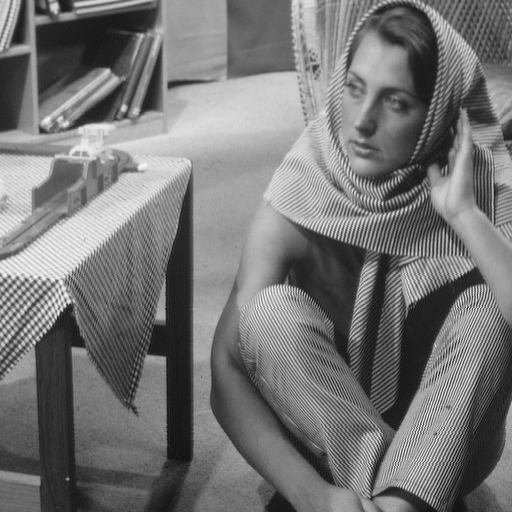
\includegraphics[scale=.35]{../images/barbara.png}
      \caption{Barbara}
    \endminipage \hfill
    \minipage{0.45\textwidth}
      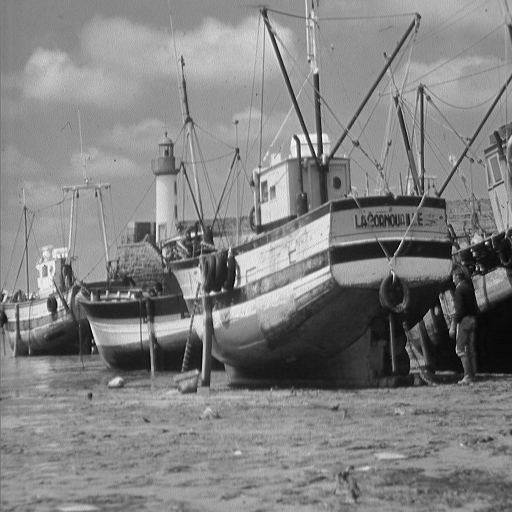
\includegraphics[scale=1.55]{../images/boat.png}
      \caption{Boat}
    \endminipage
    \end{figure}
    
    \phantom{}
    
    \begin{figure}[!htb]
    \minipage{0.45\textwidth}
      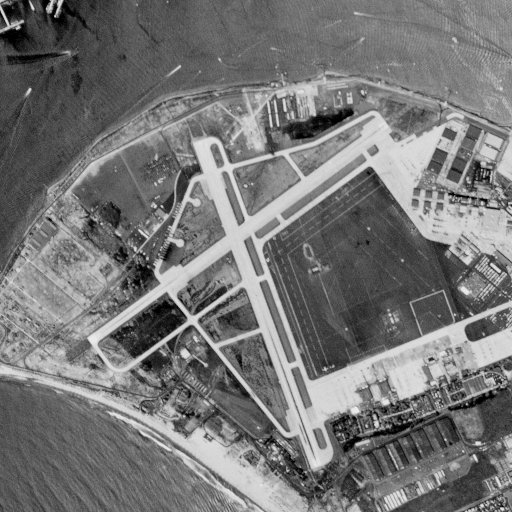
\includegraphics[scale=1.4]{../images/sandiego.png}
      \caption{Sandiego}
    \endminipage \hfill
    \minipage{0.45\textwidth}
      
\includegraphics[scale=.35]{../images/shepplogan.png}
      \caption{Shepplogan}
    \endminipage
    \end{figure}
    \pagebreak
    
% -------------------------------------------------------
% -------------------------------------------------------
% Barbara
% -------------------------------------------------------
% Gaussian
    \subsubsection*{Barbara (Gaussian)}
    
%   Image
    \begin{figure}[!htb]
    \begin{center}
     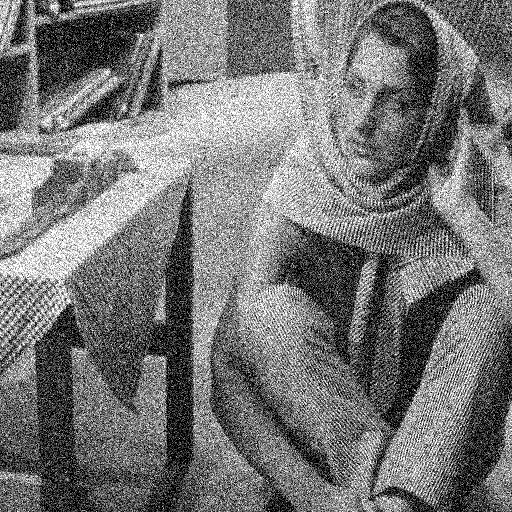
\includegraphics[scale=.3]{./basic_denoising/barbara/gaussian.png}
     \caption{Gaussian Noise}
    \end{center}
    \end{figure}
    
%   Mean Filter
    \begin{figure}[!htb]
    \minipage{0.45\textwidth}
      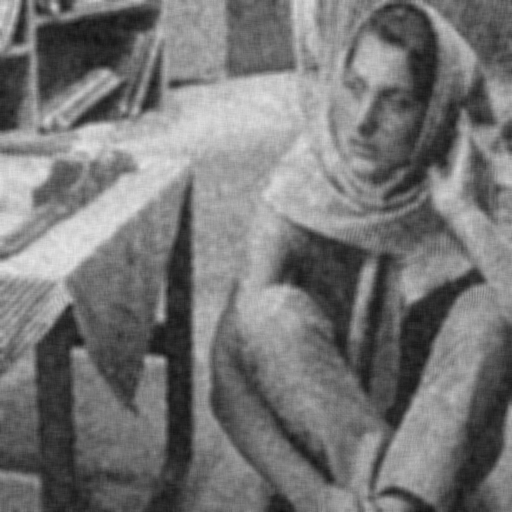
\includegraphics[scale=0.3]{./basic_denoising/barbara/average_best_gaussian.png}
      \caption{Best PSNR image (Mean)}
    \endminipage \hfill
    \minipage{0.45\textwidth}
      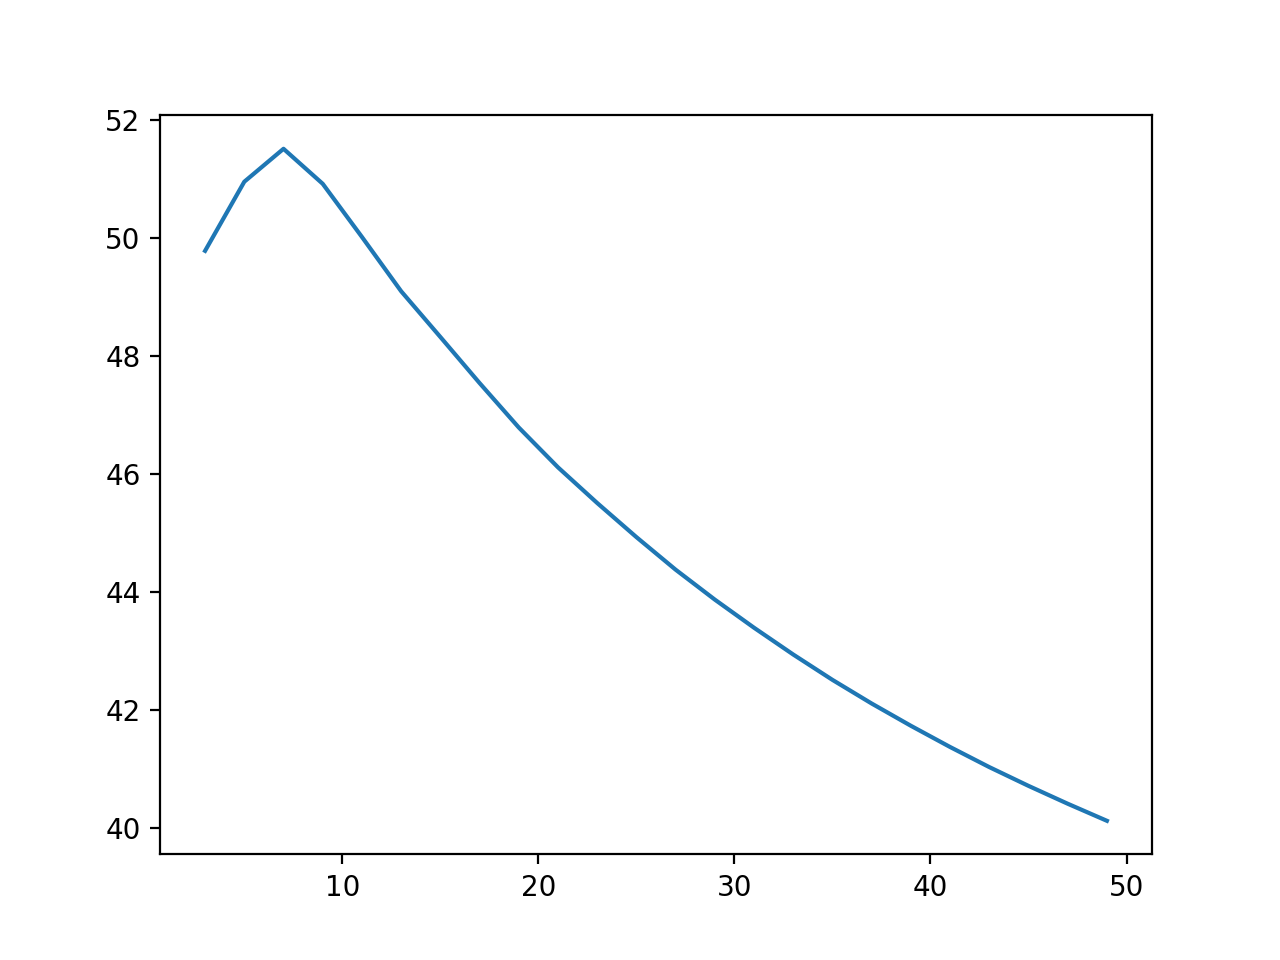
\includegraphics[scale=.45]{./basic_denoising/barbara/average_psnr_gaussian.png}
      \caption{PSNR vs filter size (Mean)}
    \endminipage
    \end{figure}
    
%   Median Filter
    \begin{figure}[!htb]
    \minipage{0.45\textwidth}
      
\includegraphics[scale=0.3]{./basic_denoising/barbara/median_best_gaussian.png}
      \caption{Best PSNR image (Median)}
    \endminipage \hfill
    \minipage{0.45\textwidth}
      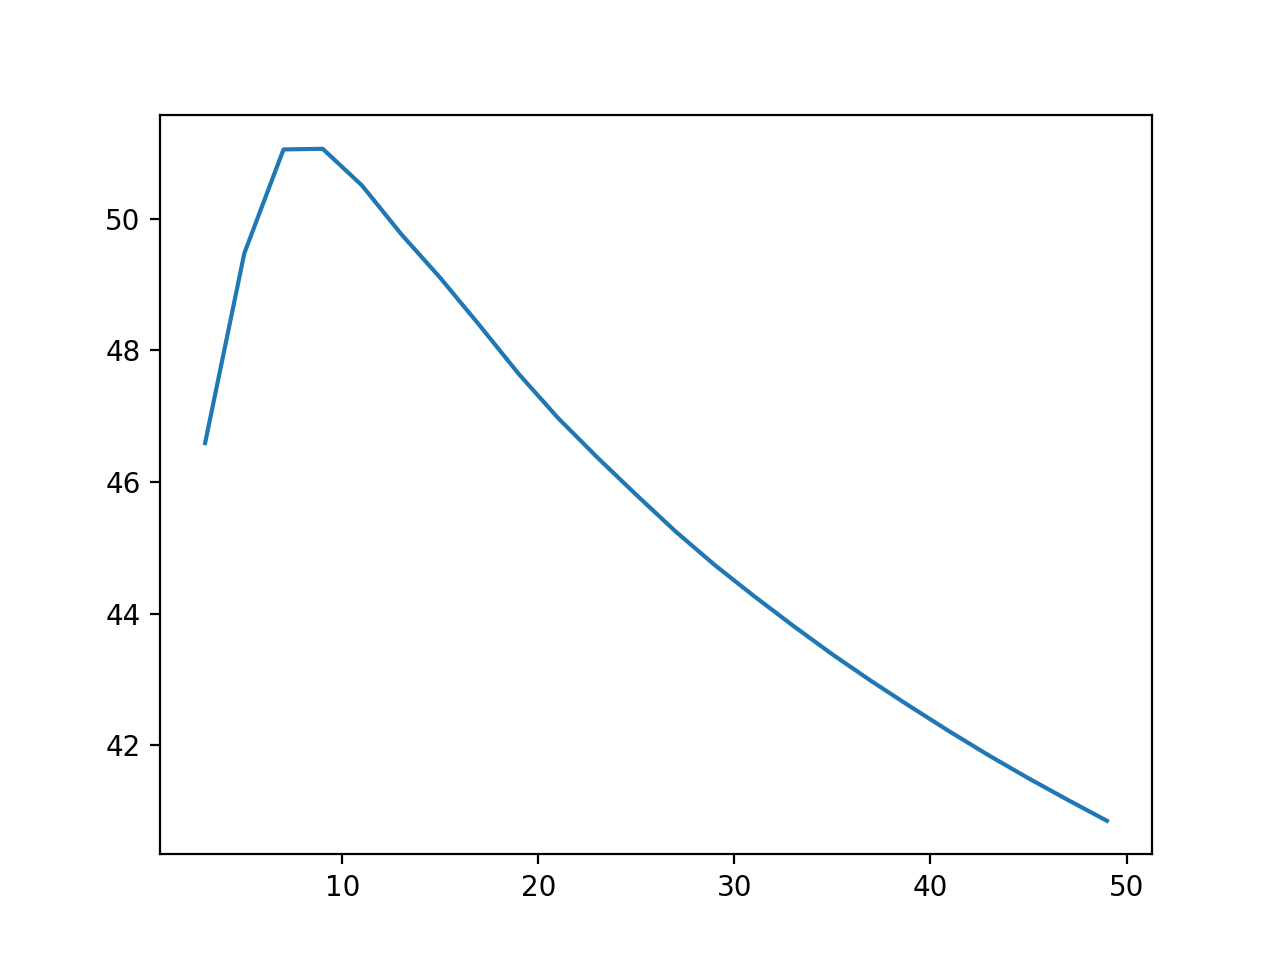
\includegraphics[scale=.45]{./basic_denoising/barbara/median_psnr_gaussian.png}
      \caption{PSNR vs filter size (Median)}
    \endminipage
    \end{figure}
    \pagebreak
% -------------------------------------------------------
% Salt\Pepper
    \subsubsection*{Barbara (Salt/Pepper)}
    
%   Image
    \begin{figure}[!htb]
    \begin{center}
     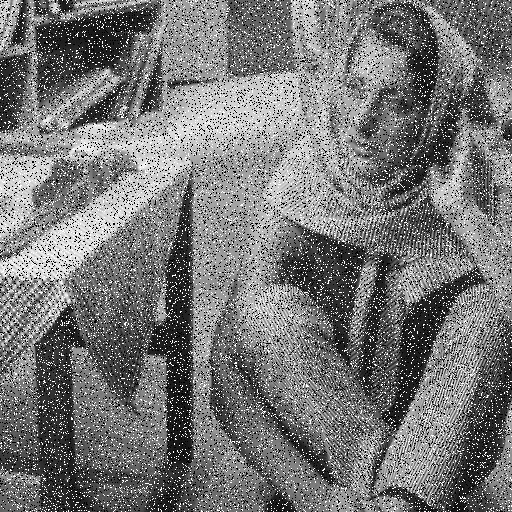
\includegraphics[scale=.3]{./basic_denoising/barbara/sp.png}
     \caption{Salt/Pepper Noise}
    \end{center}
    \end{figure}
    
%   Mean Filter
    \begin{figure}[!htb]
    \minipage{0.45\textwidth}
      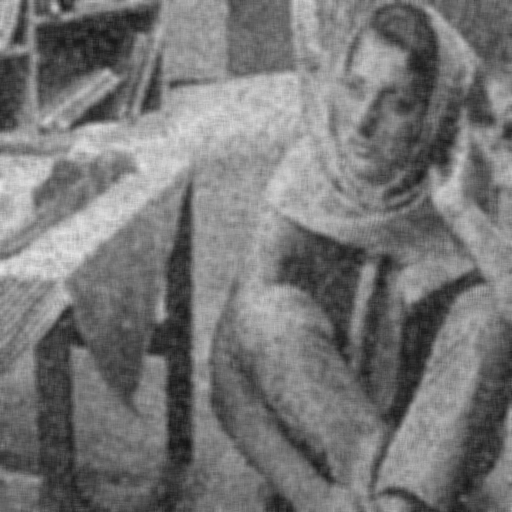
\includegraphics[scale=0.3]{./basic_denoising/barbara/average_best_sp.png}
      \caption{Best PSNR image (Mean)}
    \endminipage \hfill
    \minipage{0.45\textwidth}
      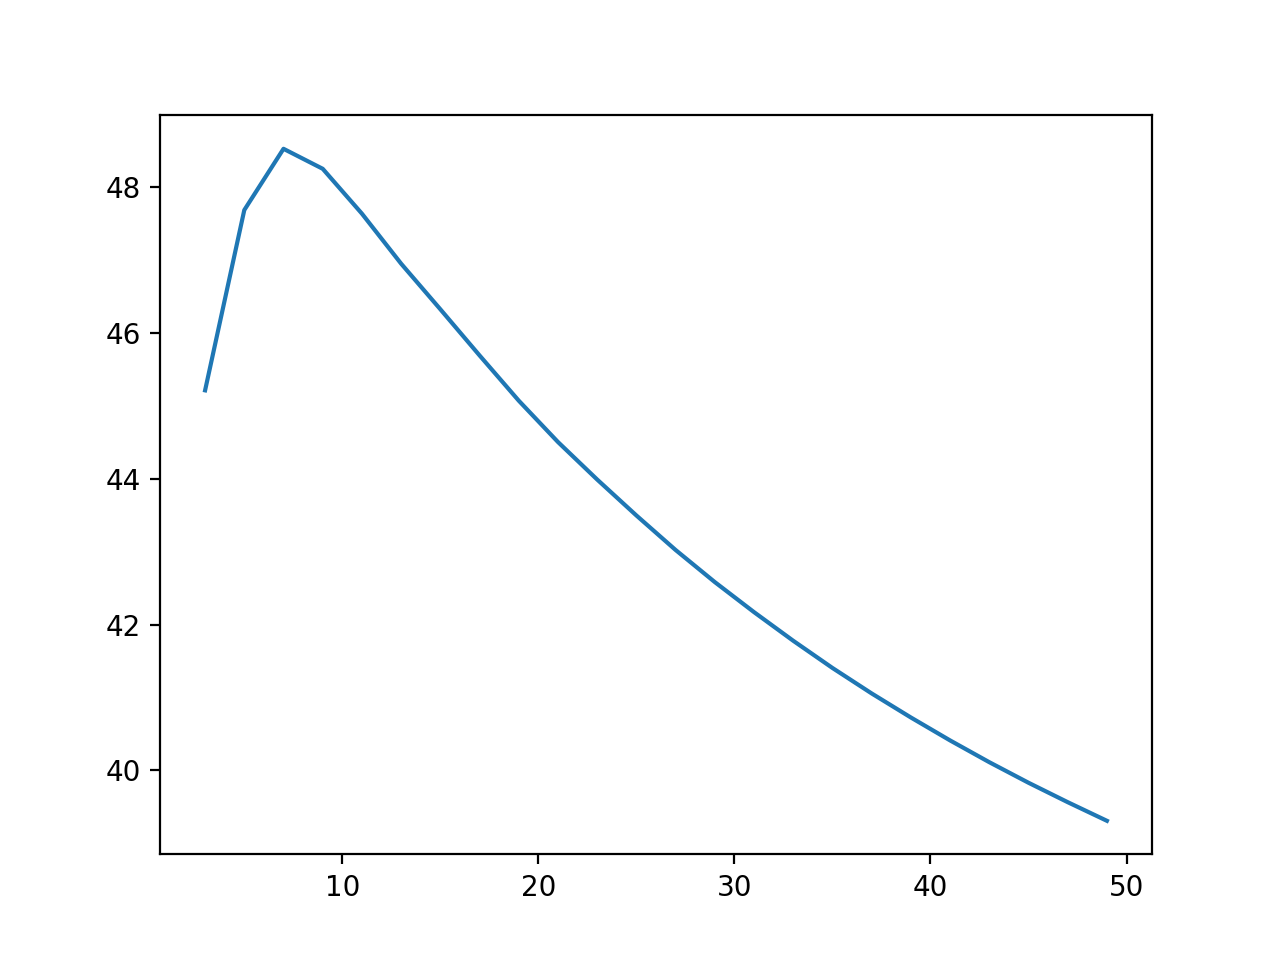
\includegraphics[scale=.45]{./basic_denoising/barbara/average_psnr_sp.png}
      \caption{PSNR vs filter size (Mean)}
    \endminipage
    \end{figure}
    
%   Median Filter
    \begin{figure}[!htb]
    \minipage{0.45\textwidth}
      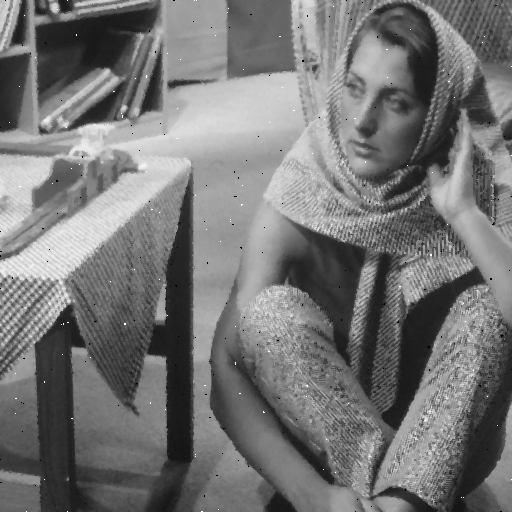
\includegraphics[scale=0.3]{./basic_denoising/barbara/median_best_sp.png}
      \caption{Best PSNR image (Median)}
    \endminipage \hfill
    \minipage{0.45\textwidth}
      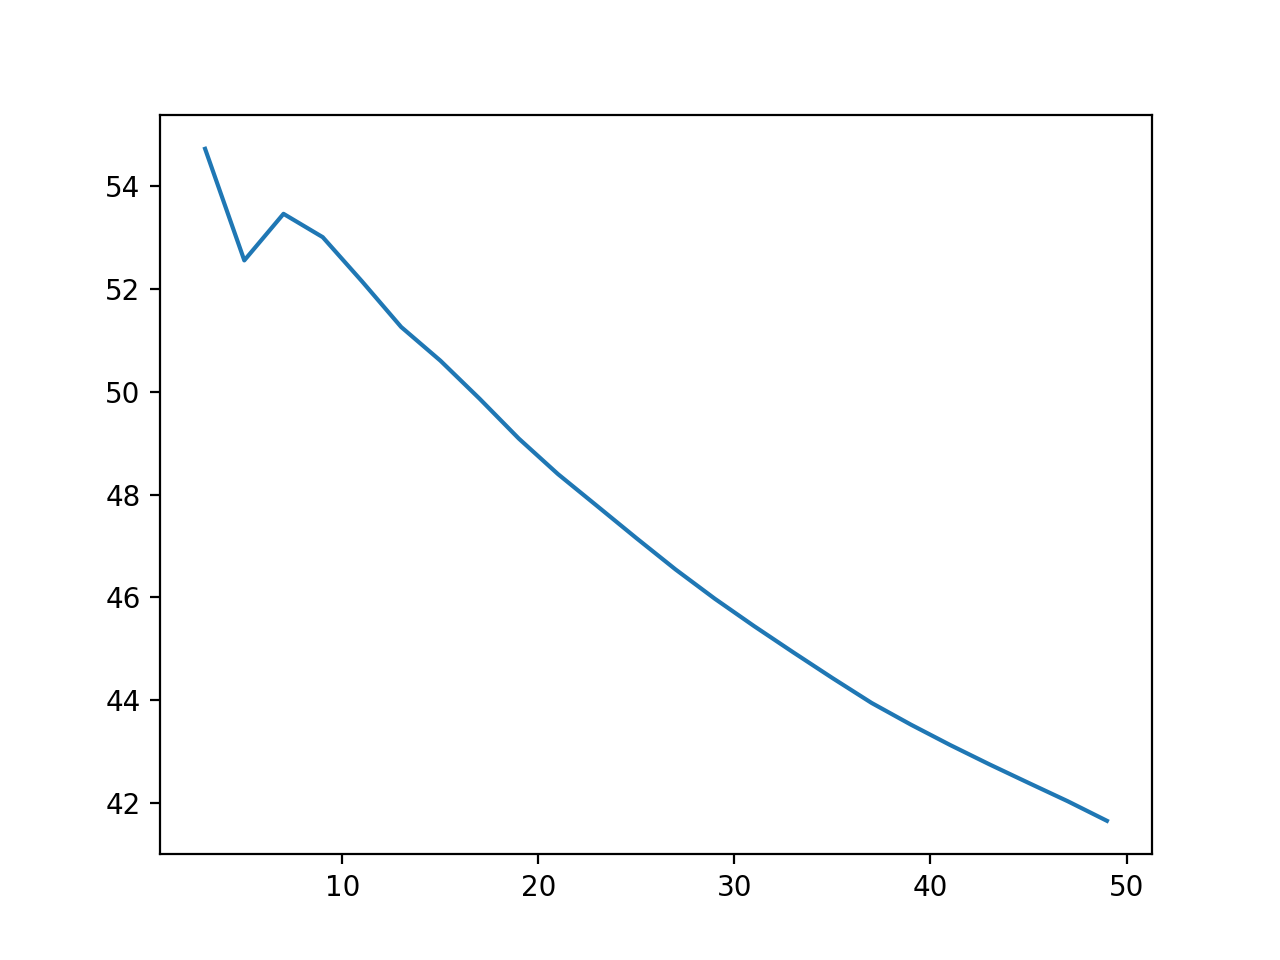
\includegraphics[scale=.45]{./basic_denoising/barbara/median_psnr_sp.png}
      \caption{PSNR vs filter size (Median)}
    \endminipage
    \end{figure}
    \pagebreak
% -------------------------------------------------------
% Complete
    
% -------------------------------------------------------
% -------------------------------------------------------
% Boat
% -------------------------------------------------------
% Gaussian
    \subsubsection*{Boat (Gaussian)}
    
%   Image
    \begin{figure}[!htb]
    \begin{center}
     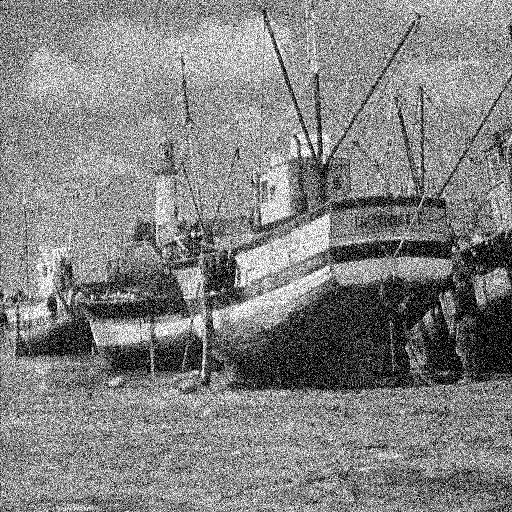
\includegraphics[scale=.3]{./basic_denoising/boat/gaussian.png}
     \caption{Gaussian Noise}
    \end{center}
    \end{figure}
    
%   Mean Filter
    \begin{figure}[!htb]
    \minipage{0.45\textwidth}
      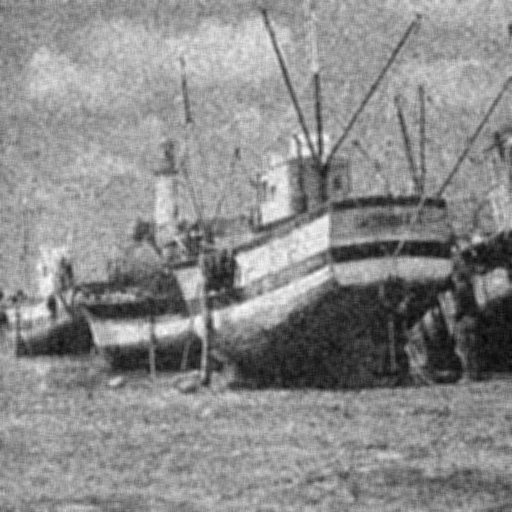
\includegraphics[scale=0.3]{./basic_denoising/boat/average_best_gaussian.png}
      \caption{Best PSNR image (Mean)}
    \endminipage \hfill
    \minipage{0.45\textwidth}
      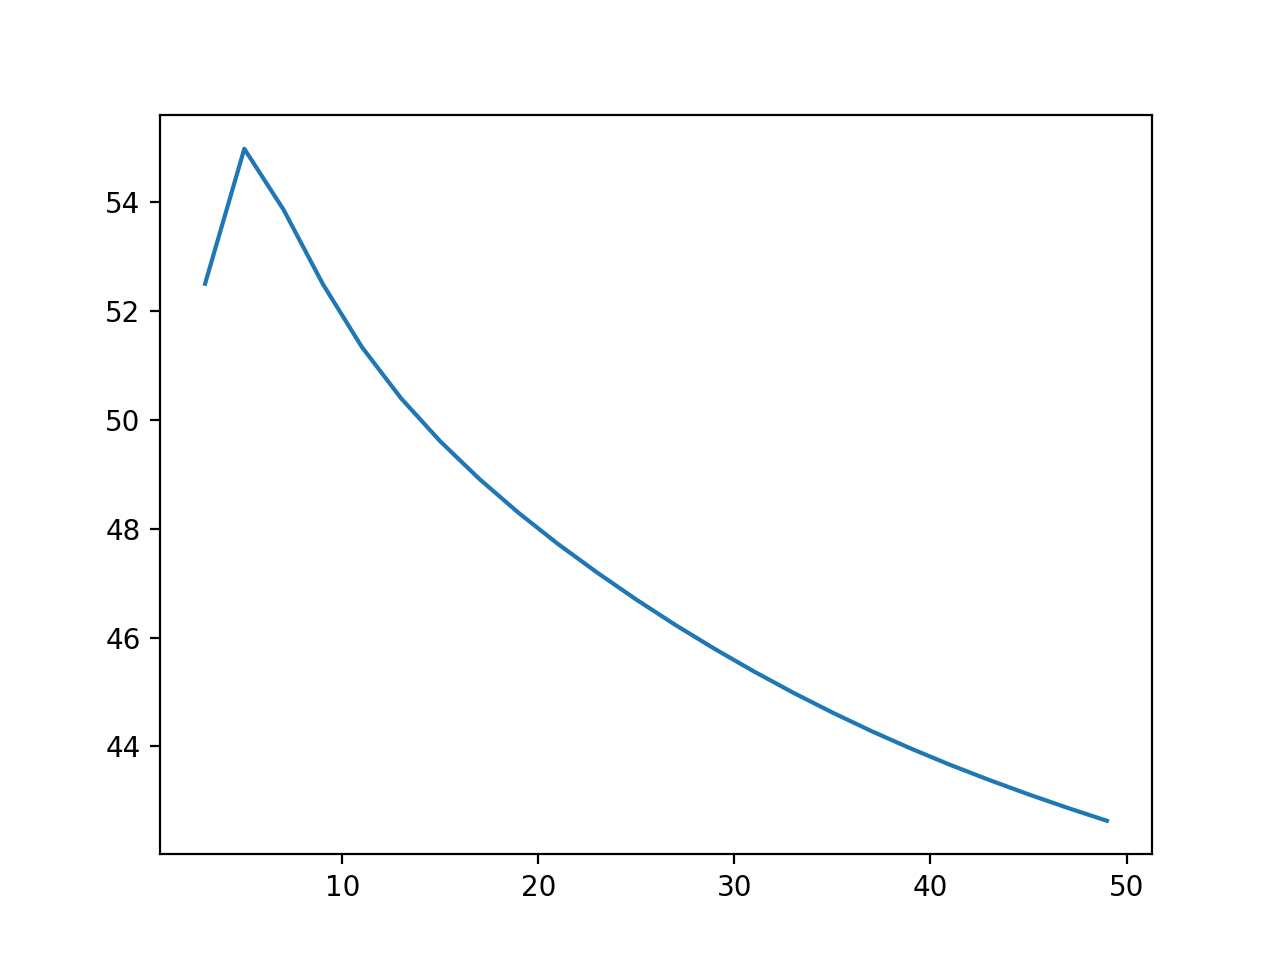
\includegraphics[scale=.45]{./basic_denoising/boat/average_psnr_gaussian.png}
      \caption{PSNR vs filter size (Mean)}
    \endminipage
    \end{figure}
    
%   Median Filter
    \begin{figure}[!htb]
    \minipage{0.45\textwidth}
      
\includegraphics[scale=0.3]{./basic_denoising/boat/median_best_gaussian.png}
      \caption{Best PSNR image (Median)}
    \endminipage \hfill
    \minipage{0.45\textwidth}
      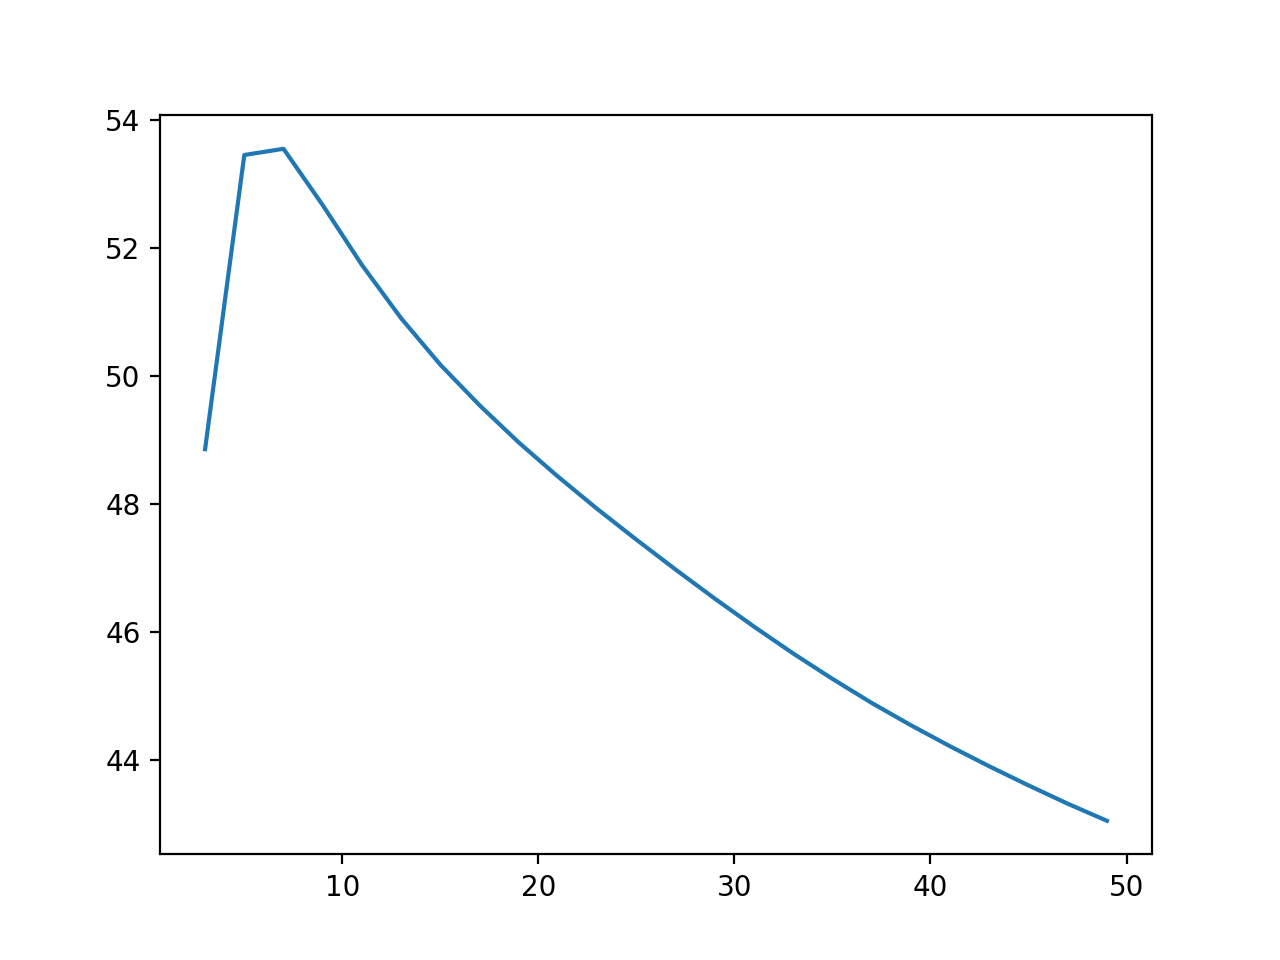
\includegraphics[scale=.45]{./basic_denoising/boat/median_psnr_gaussian.png}
      \caption{PSNR vs filter size (Median)}
    \endminipage
    \end{figure}
    \pagebreak
% -------------------------------------------------------
% Salt\Pepper
    \subsubsection*{Boat (Salt/Pepper)}
    
%   Image
    \begin{figure}[!htb]
    \begin{center}
     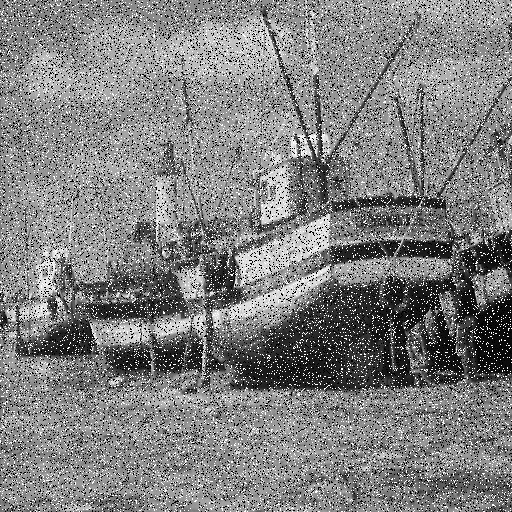
\includegraphics[scale=.3]{./basic_denoising/boat/sp.png}
     \caption{Salt/Pepper Noise}
    \end{center}
    \end{figure}
    
%   Mean Filter
    \begin{figure}[!htb]
    \minipage{0.45\textwidth}
      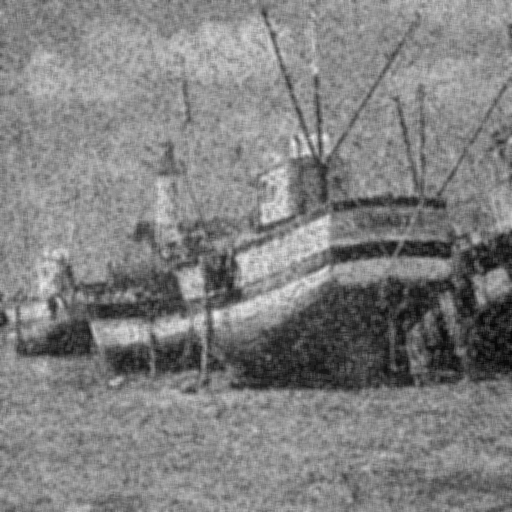
\includegraphics[scale=0.3]{./basic_denoising/boat/average_best_sp.png}
      \caption{Best PSNR image (Mean)}
    \endminipage \hfill
    \minipage{0.45\textwidth}
      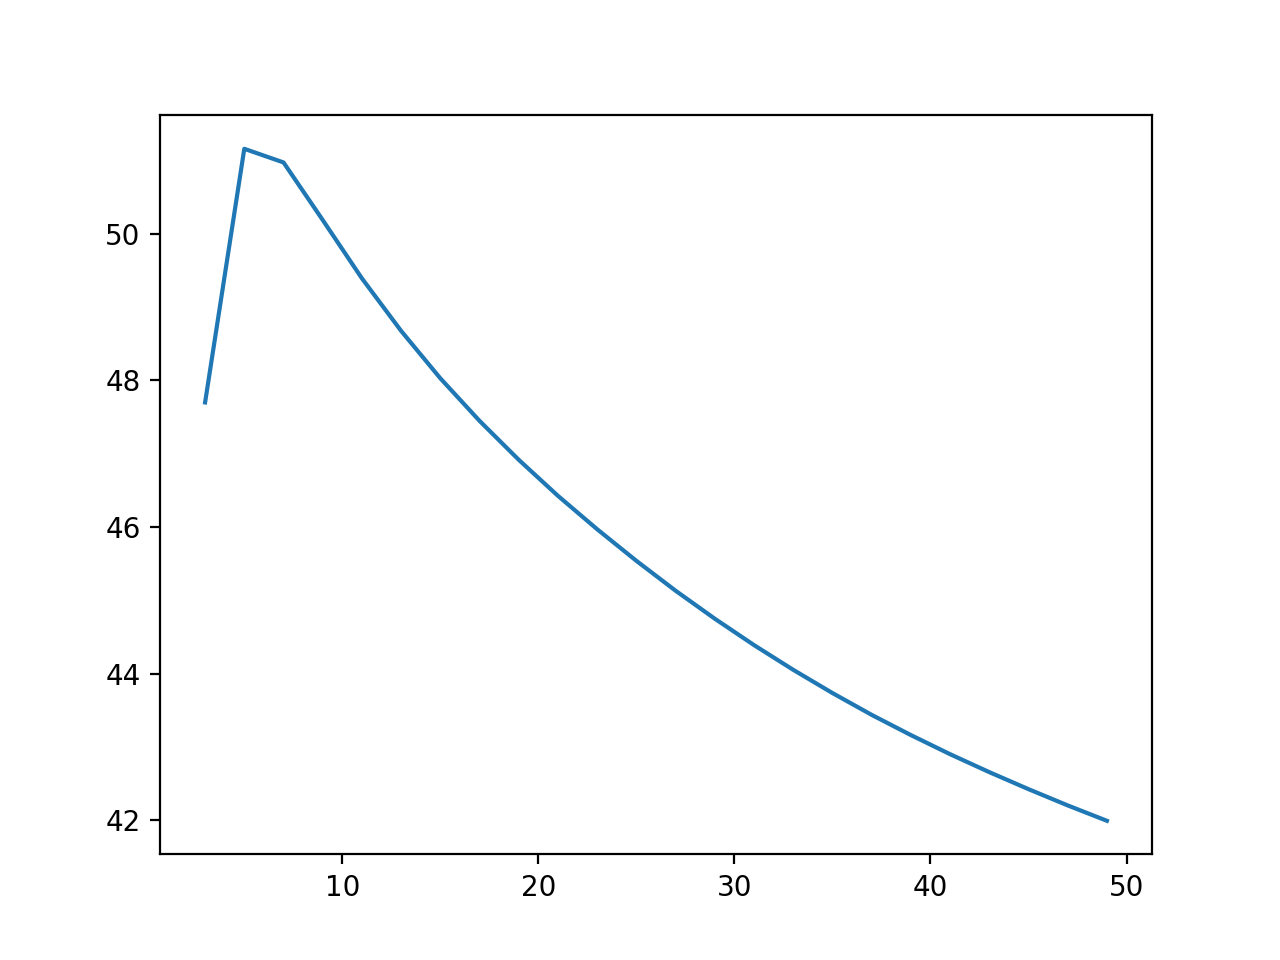
\includegraphics[scale=.45]{./basic_denoising/boat/average_psnr_sp.png}
      \caption{PSNR vs filter size (Mean)}
    \endminipage
    \end{figure}
    
%   Median Filter
    \begin{figure}[!htb]
    \minipage{0.45\textwidth}
      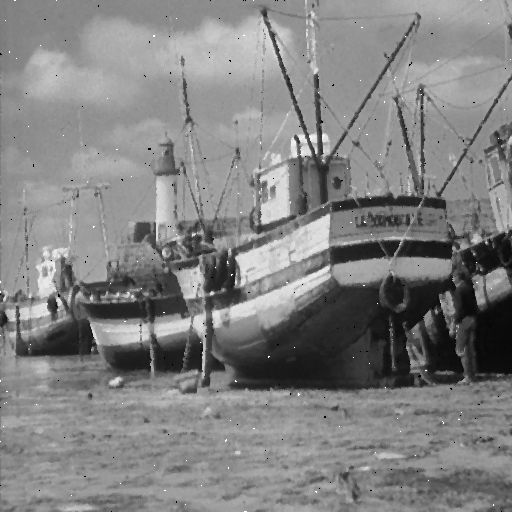
\includegraphics[scale=0.3]{./basic_denoising/boat/median_best_sp.png}
      \caption{Best PSNR image (Median)}
    \endminipage \hfill
    \minipage{0.45\textwidth}
      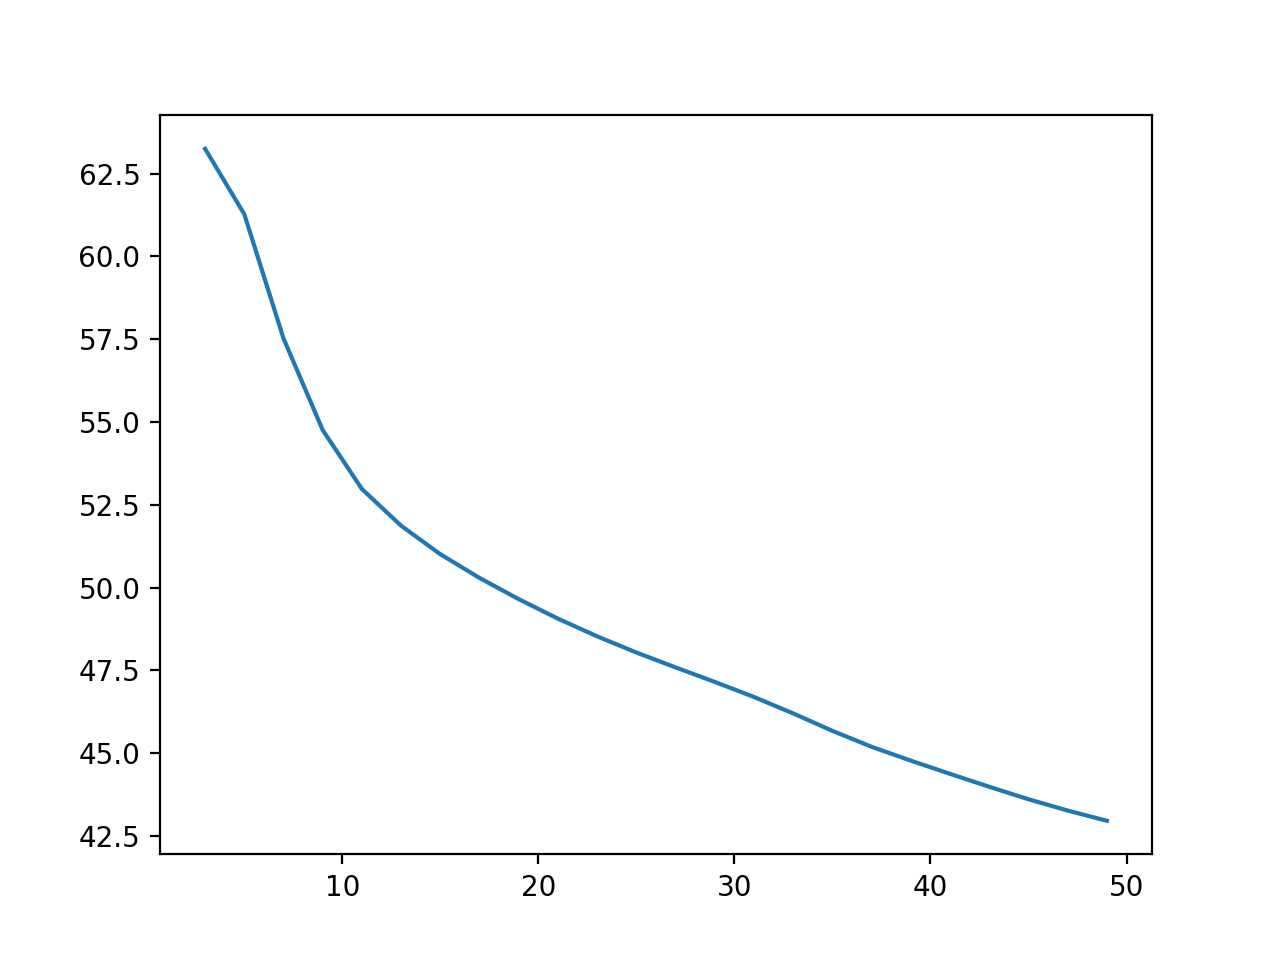
\includegraphics[scale=.45]{./basic_denoising/boat/median_psnr_sp.png}
      \caption{PSNR vs filter size (Median)}
    \endminipage
    \end{figure}
    \pagebreak
% -------------------------------------------------------
% Complete

% -------------------------------------------------------
% -------------------------------------------------------
% Sandiego
% -------------------------------------------------------
% Gaussian
    \subsubsection*{Sandiego (Gaussian)}
    
%   Image
    \begin{figure}[!htb]
    \begin{center}
     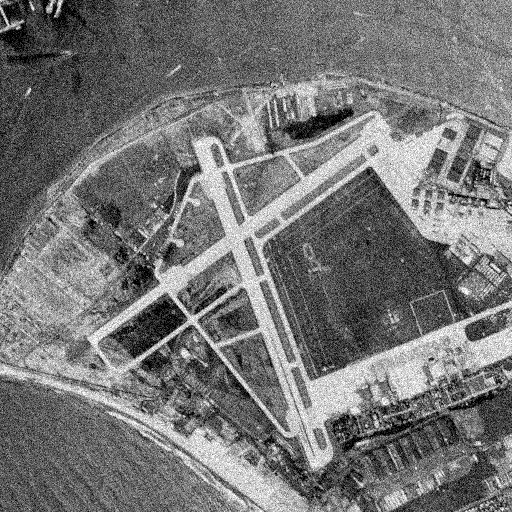
\includegraphics[scale=.3]{./basic_denoising/sandiego/gaussian.png}
     \caption{Gaussian Noise}
    \end{center}
    \end{figure}
    
%   Mean Filter
    \begin{figure}[!htb]
    \minipage{0.45\textwidth}
      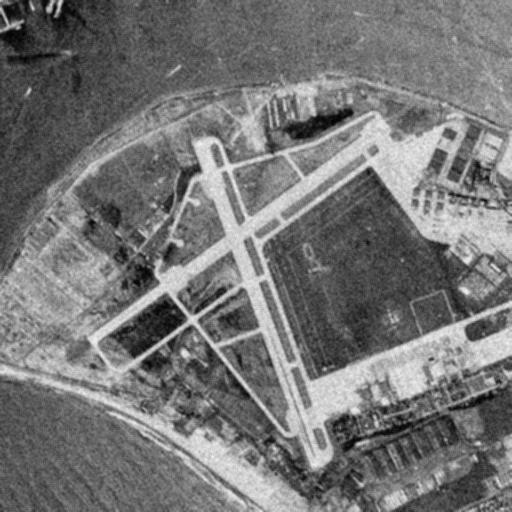
\includegraphics[scale=0.3]{./basic_denoising/sandiego/average_best_gaussian.png}
      \caption{Best PSNR image (Mean)}
    \endminipage \hfill
    \minipage{0.45\textwidth}
      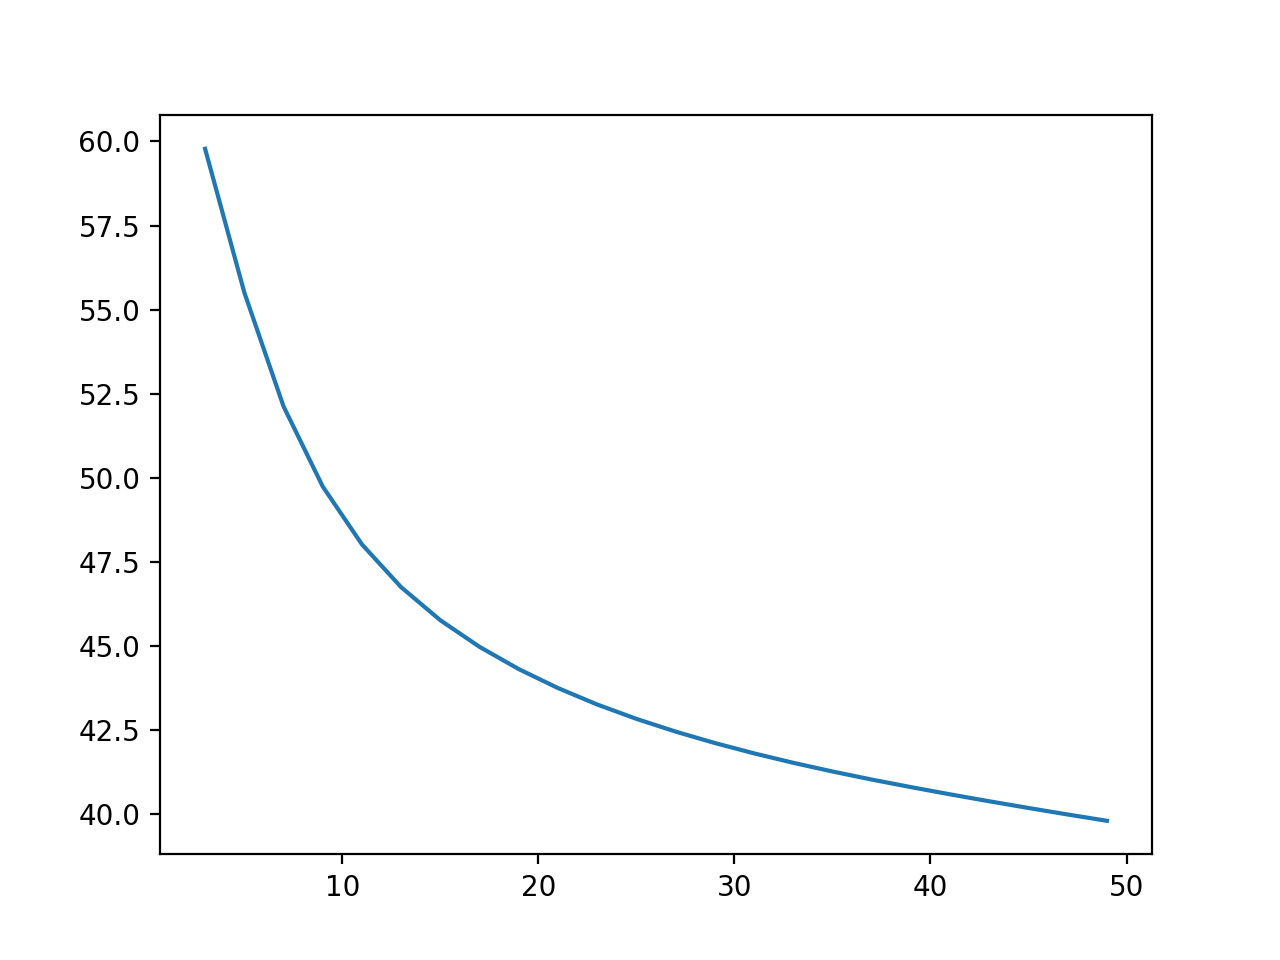
\includegraphics[scale=.45]{./basic_denoising/sandiego/average_psnr_gaussian.png}
      \caption{PSNR vs filter size (Mean)}
    \endminipage
    \end{figure}
    
%   Median Filter
    \begin{figure}[!htb]
    \minipage{0.45\textwidth}
      
\includegraphics[scale=0.3]{./basic_denoising/sandiego/median_best_gaussian.png}
      \caption{Best PSNR image (Median)}
    \endminipage \hfill
    \minipage{0.45\textwidth}
      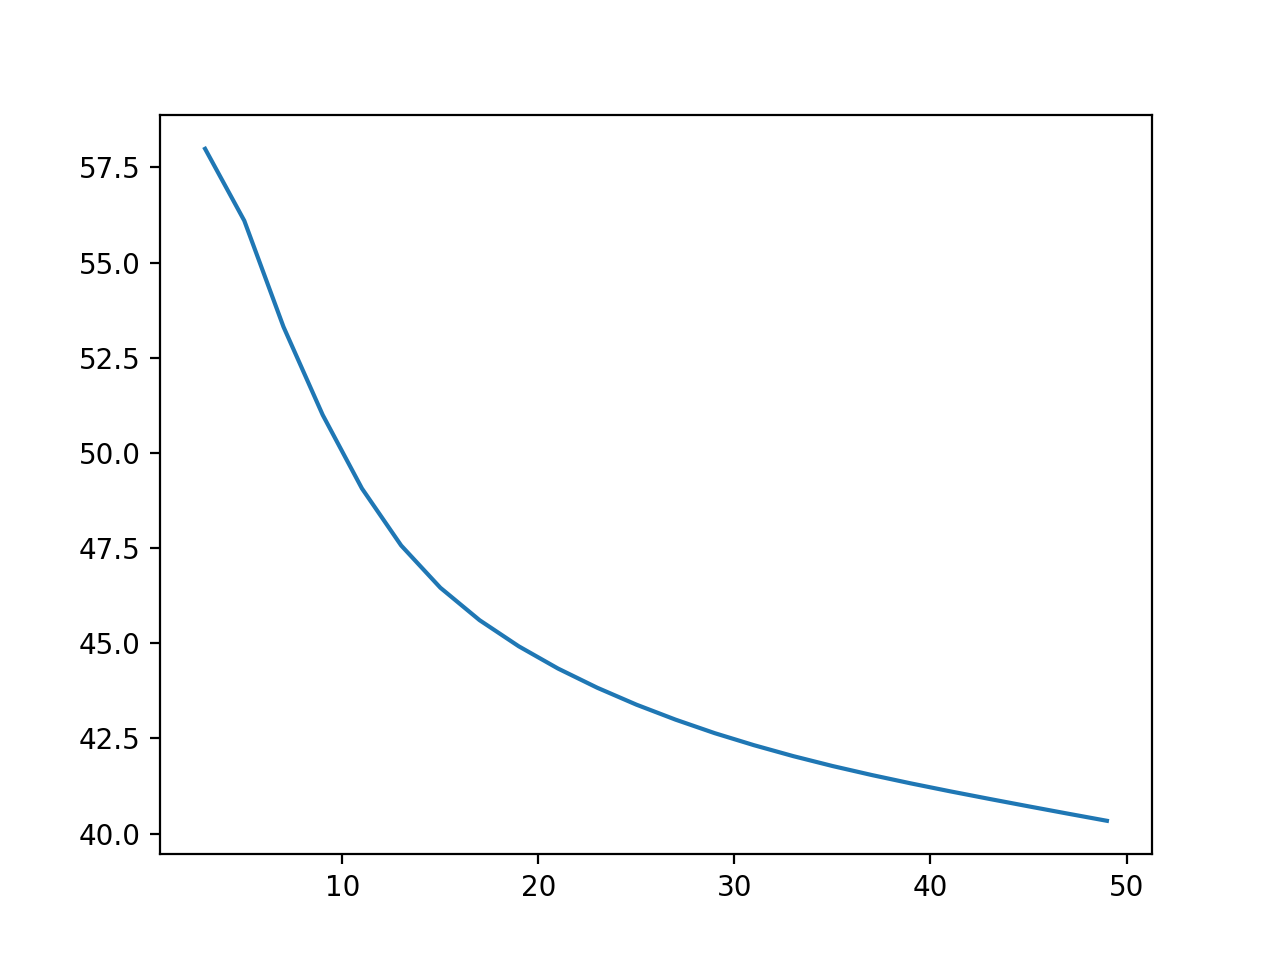
\includegraphics[scale=.45]{./basic_denoising/sandiego/median_psnr_gaussian.png}
      \caption{PSNR vs filter size (Median)}
    \endminipage
    \end{figure}
    \pagebreak
% -------------------------------------------------------
% Salt\Pepper
    \subsubsection*{Sandiego (Salt/Pepper)}
    
%   Image
    \begin{figure}[!htb]
    \begin{center}
     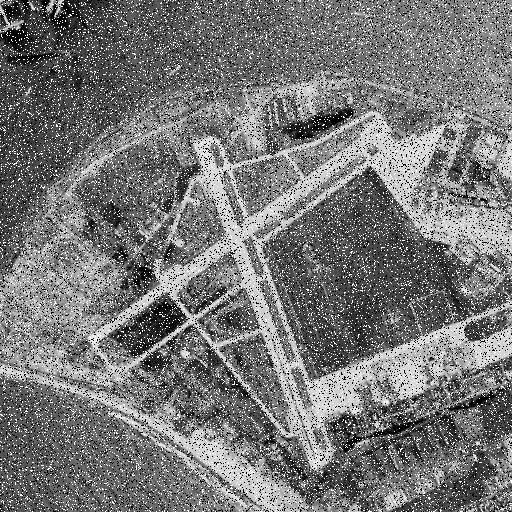
\includegraphics[scale=.3]{./basic_denoising/sandiego/sp.png}
     \caption{Salt/Pepper Noise}
    \end{center}
    \end{figure}
    
%   Mean Filter
    \begin{figure}[!htb]
    \minipage{0.45\textwidth}
      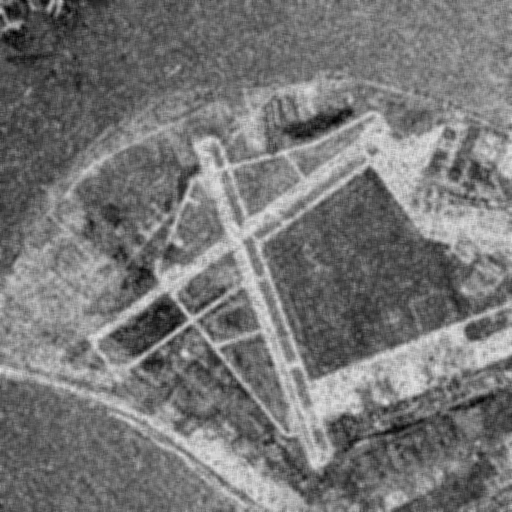
\includegraphics[scale=0.3]{./basic_denoising/sandiego/average_best_sp.png}
      \caption{Best PSNR image (Mean)}
    \endminipage \hfill
    \minipage{0.45\textwidth}
      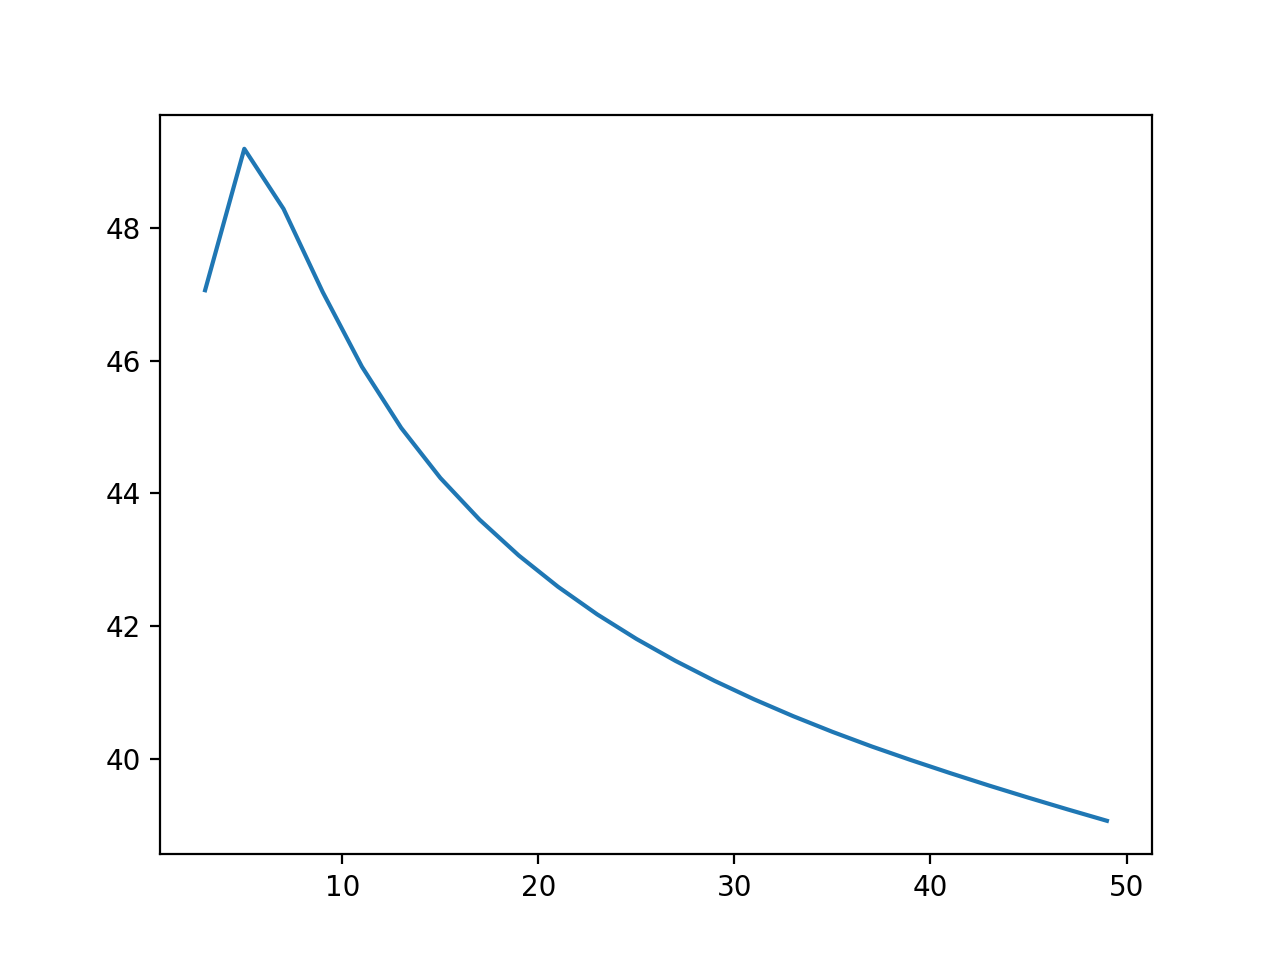
\includegraphics[scale=.45]{./basic_denoising/sandiego/average_psnr_sp.png}
      \caption{PSNR vs filter size (Mean)}
    \endminipage
    \end{figure}
    
%   Median Filter
    \begin{figure}[!htb]
    \minipage{0.45\textwidth}
      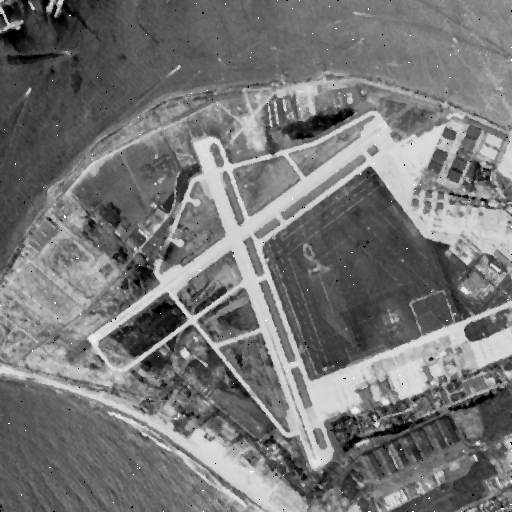
\includegraphics[scale=0.3]{./basic_denoising/sandiego/median_best_sp.png}
      \caption{Best PSNR image (Median)}
    \endminipage \hfill
    \minipage{0.45\textwidth}
      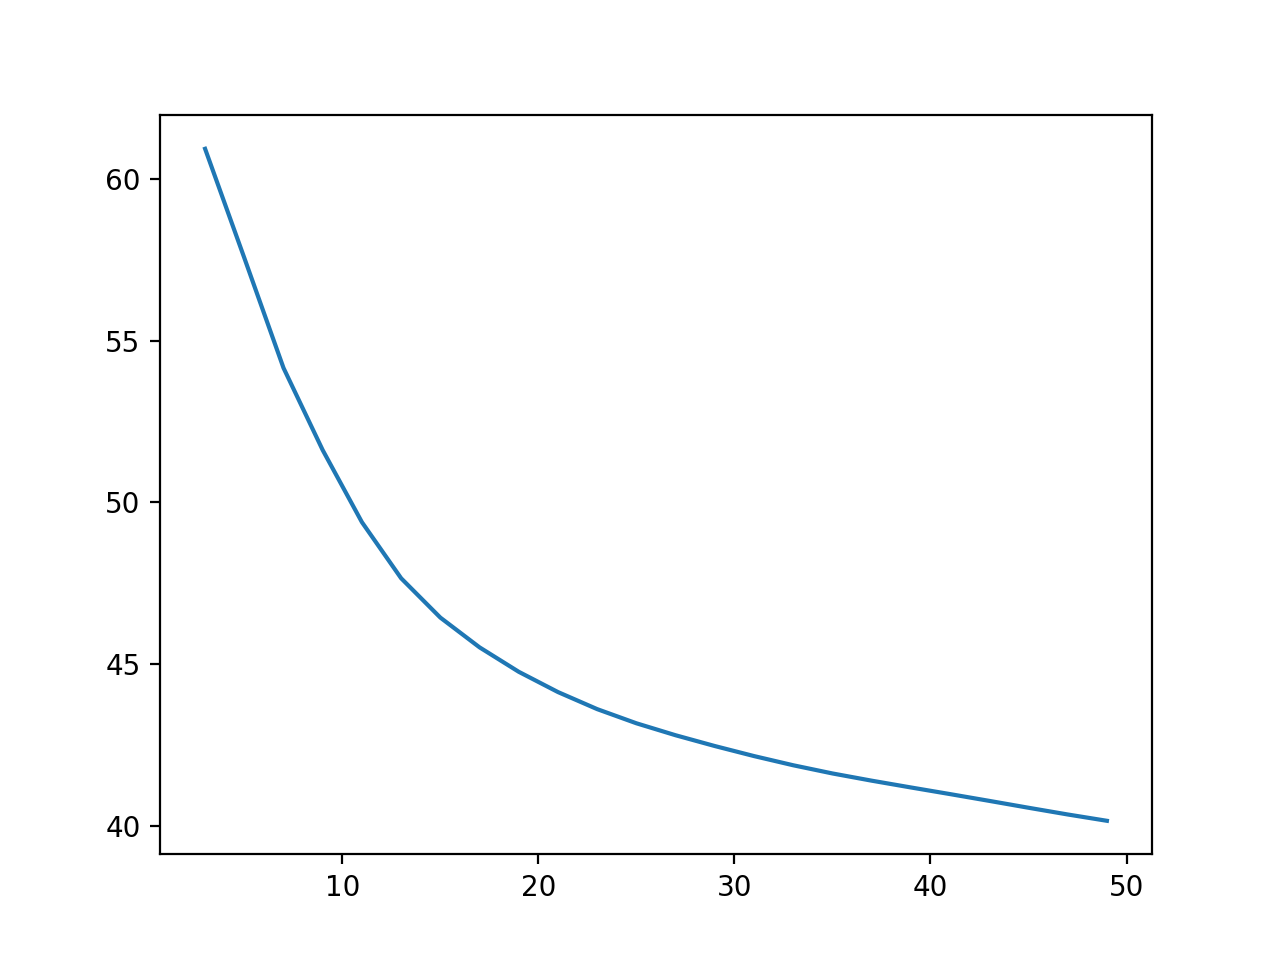
\includegraphics[scale=.45]{./basic_denoising/sandiego/median_psnr_sp.png}
      \caption{PSNR vs filter size (Median)}
    \endminipage
    \end{figure}
    \pagebreak
% -------------------------------------------------------
% Complete

% -------------------------------------------------------
% -------------------------------------------------------
% Shepplogan
% -------------------------------------------------------
% Gaussian
    \subsubsection*{Shepplogan (Gaussian)}
    
%   Image
    \begin{figure}[!htb]
    \begin{center}
     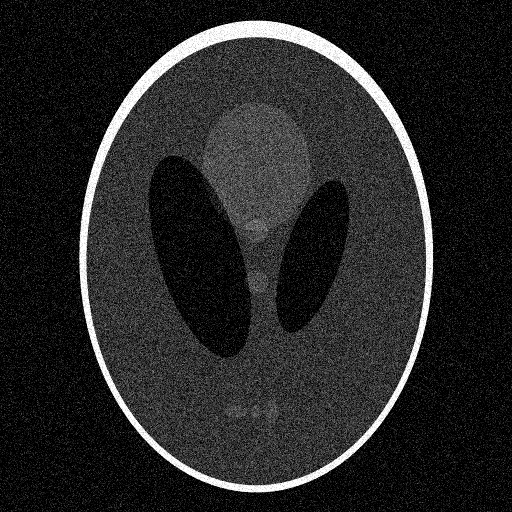
\includegraphics[scale=.3]{./basic_denoising/shepplogan/gaussian.png}
     \caption{Gaussian Noise}
    \end{center}
    \end{figure}
    
%   Mean Filter
    \begin{figure}[!htb]
    \minipage{0.45\textwidth}
      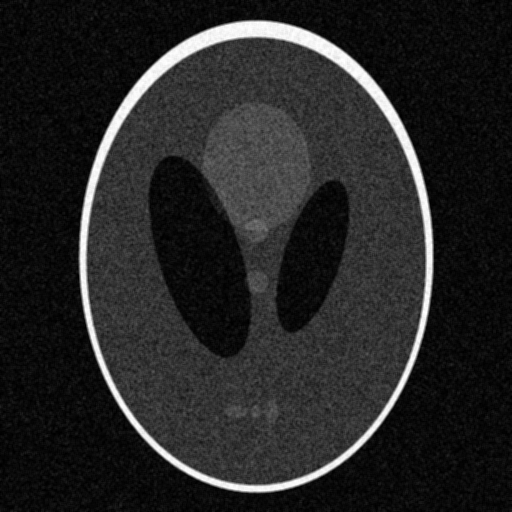
\includegraphics[scale=0.3]{./basic_denoising/shepplogan/average_best_gaussian.png}
      \caption{Best PSNR image (Mean)}
    \endminipage \hfill
    \minipage{0.45\textwidth}
      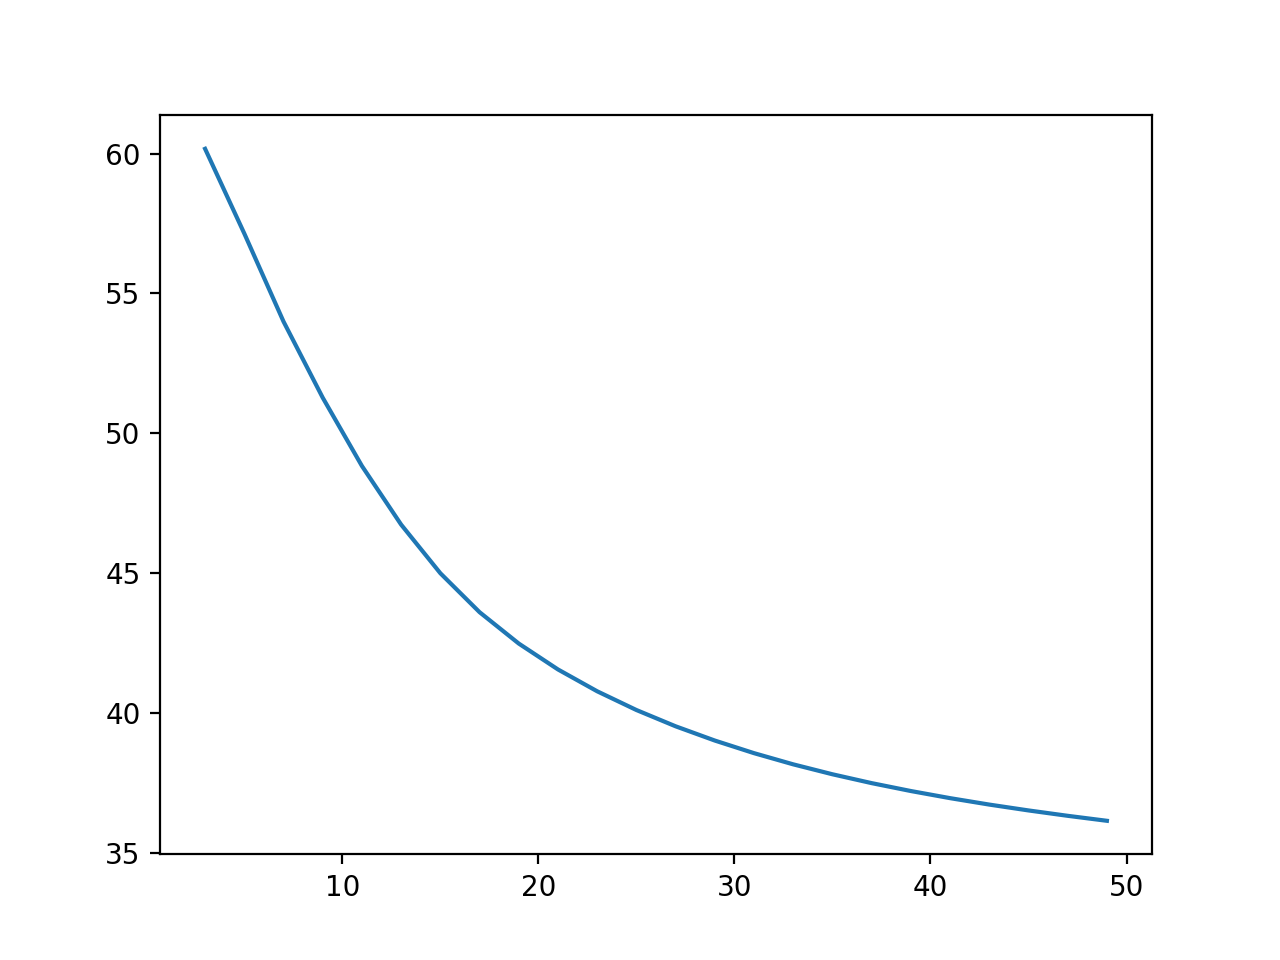
\includegraphics[scale=.45]{./basic_denoising/shepplogan/average_psnr_gaussian.png}
      \caption{PSNR vs filter size (Mean)}
    \endminipage
    \end{figure}
    
%   Median Filter
    \begin{figure}[!htb]
    \minipage{0.45\textwidth}
      
\includegraphics[scale=0.3]{./basic_denoising/shepplogan/median_best_gaussian.png}
      \caption{Best PSNR image (Median)}
    \endminipage \hfill
    \minipage{0.45\textwidth}
      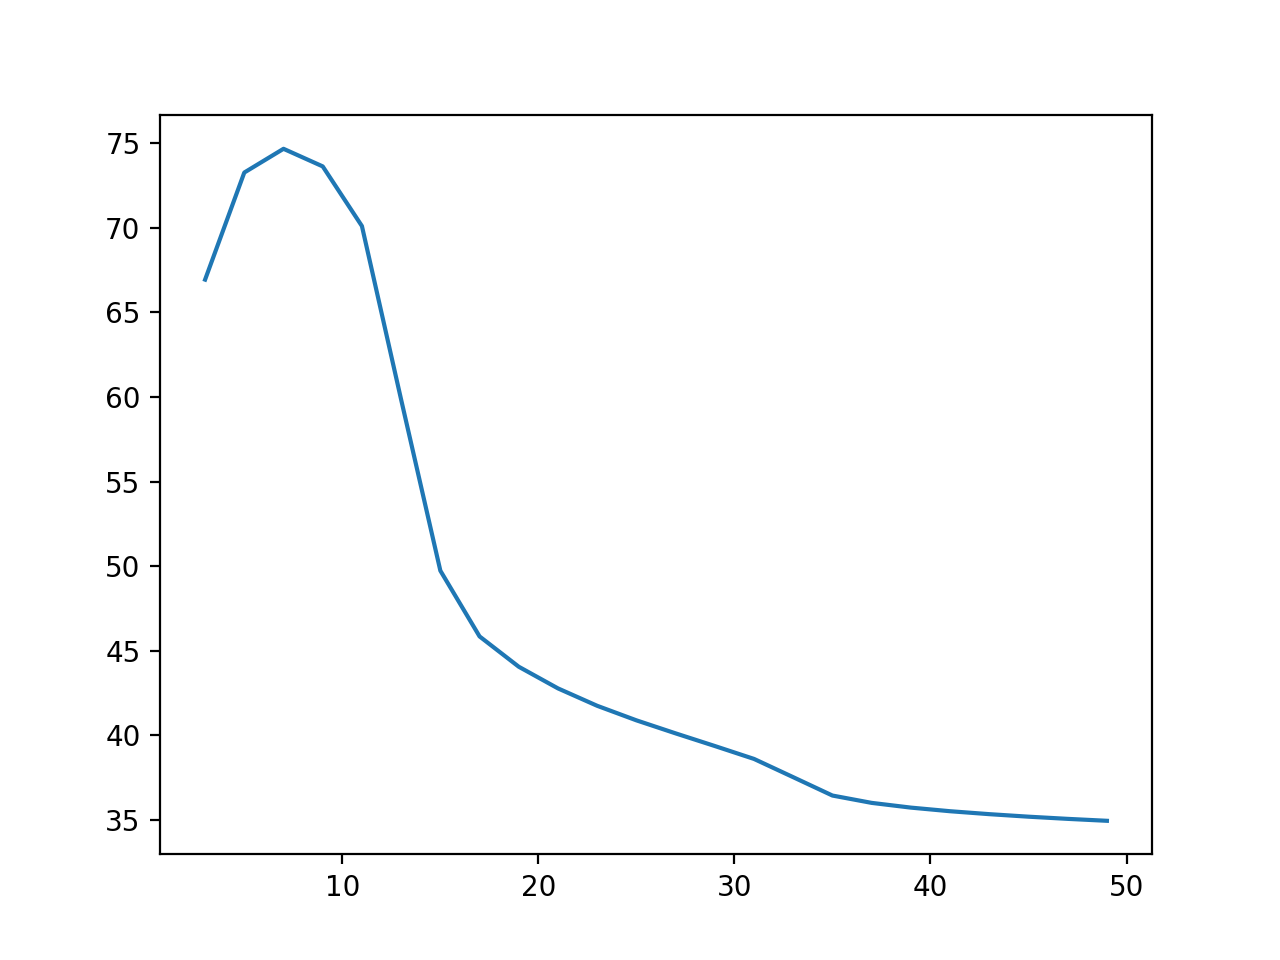
\includegraphics[scale=.45]{./basic_denoising/shepplogan/median_psnr_gaussian.png}
      \caption{PSNR vs filter size (Median)}
    \endminipage
    \end{figure}
    \pagebreak
% -------------------------------------------------------
% Salt\Pepper
    \subsubsection*{Shepplogan (Salt/Pepper)}
    
%   Image
    \begin{figure}[!htb]
    \begin{center}
     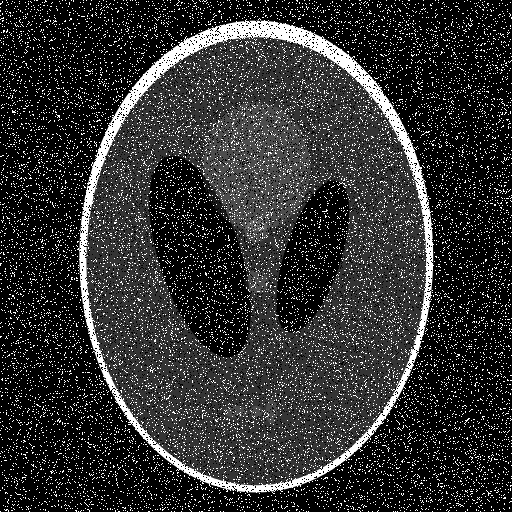
\includegraphics[scale=.3]{./basic_denoising/shepplogan/sp.png}
     \caption{Salt/Pepper Noise}
    \end{center}
    \end{figure}
    
%   Mean Filter
    \begin{figure}[!htb]
    \minipage{0.45\textwidth}
      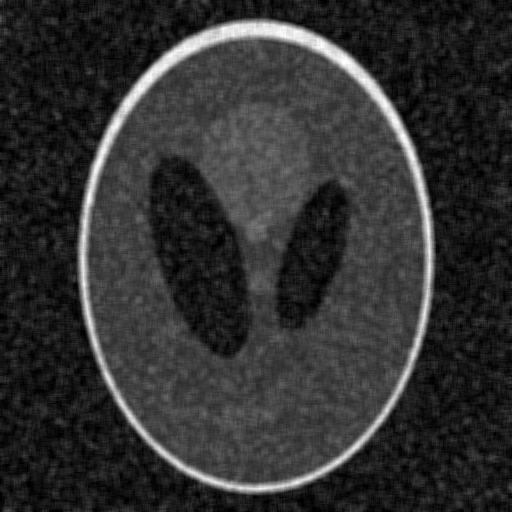
\includegraphics[scale=0.3]{./basic_denoising/shepplogan/average_best_sp.png}
      \caption{Best PSNR image (Mean)}
    \endminipage \hfill
    \minipage{0.45\textwidth}
      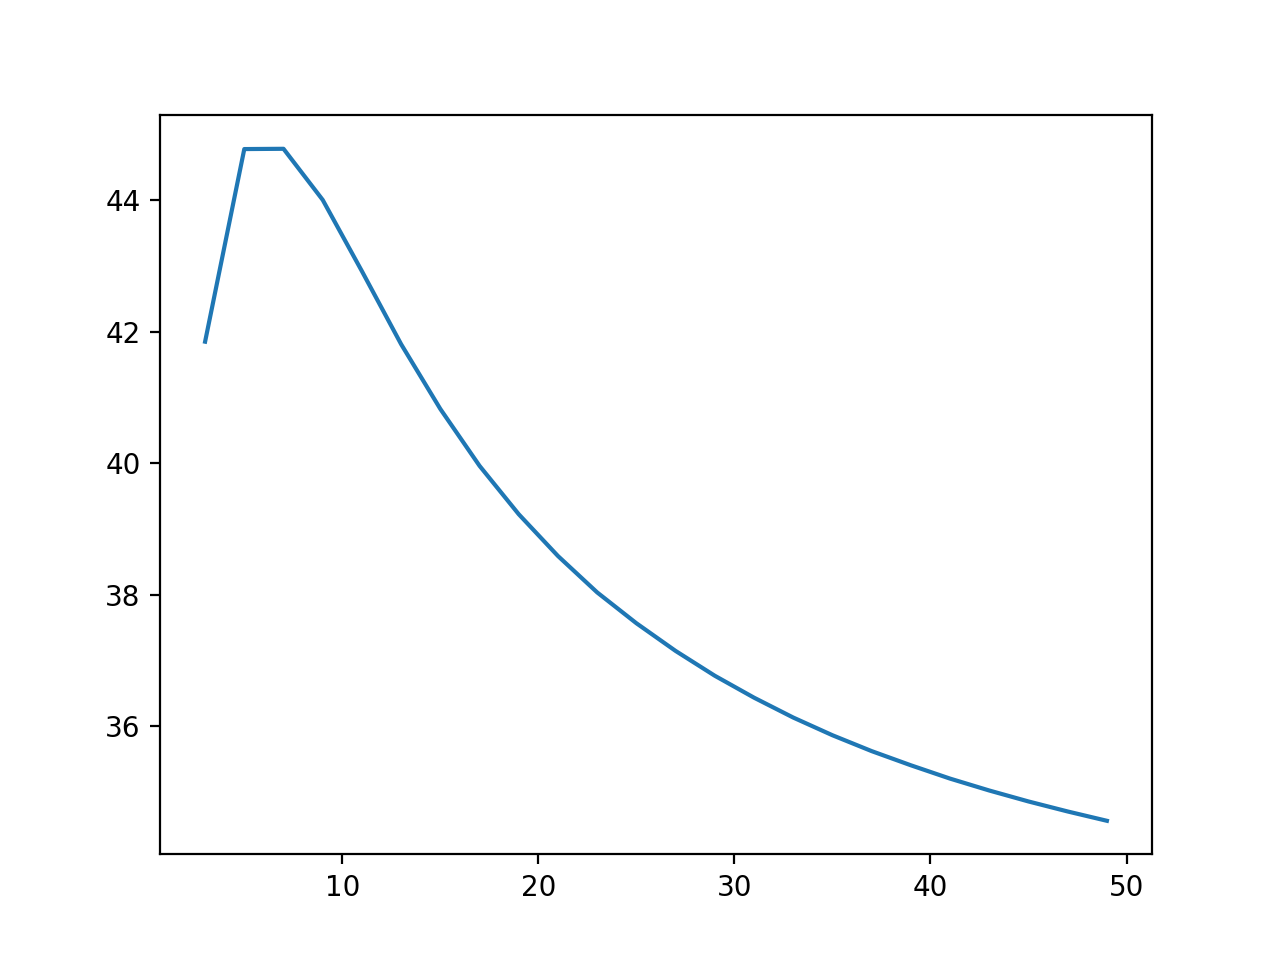
\includegraphics[scale=.45]{./basic_denoising/shepplogan/average_psnr_sp.png}
      \caption{PSNR vs filter size (Mean)}
    \endminipage
    \end{figure}
    
%   Median Filter
    \begin{figure}[!htb]
    \minipage{0.45\textwidth}
      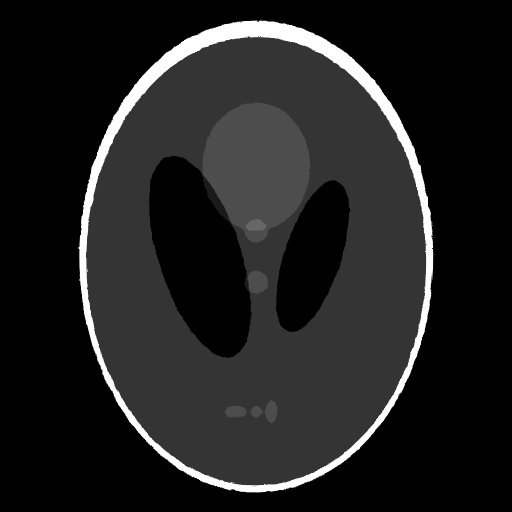
\includegraphics[scale=0.3]{./basic_denoising/shepplogan/median_best_sp.png}
      \caption{Best PSNR image (Median)}
    \endminipage \hfill
    \minipage{0.45\textwidth}
      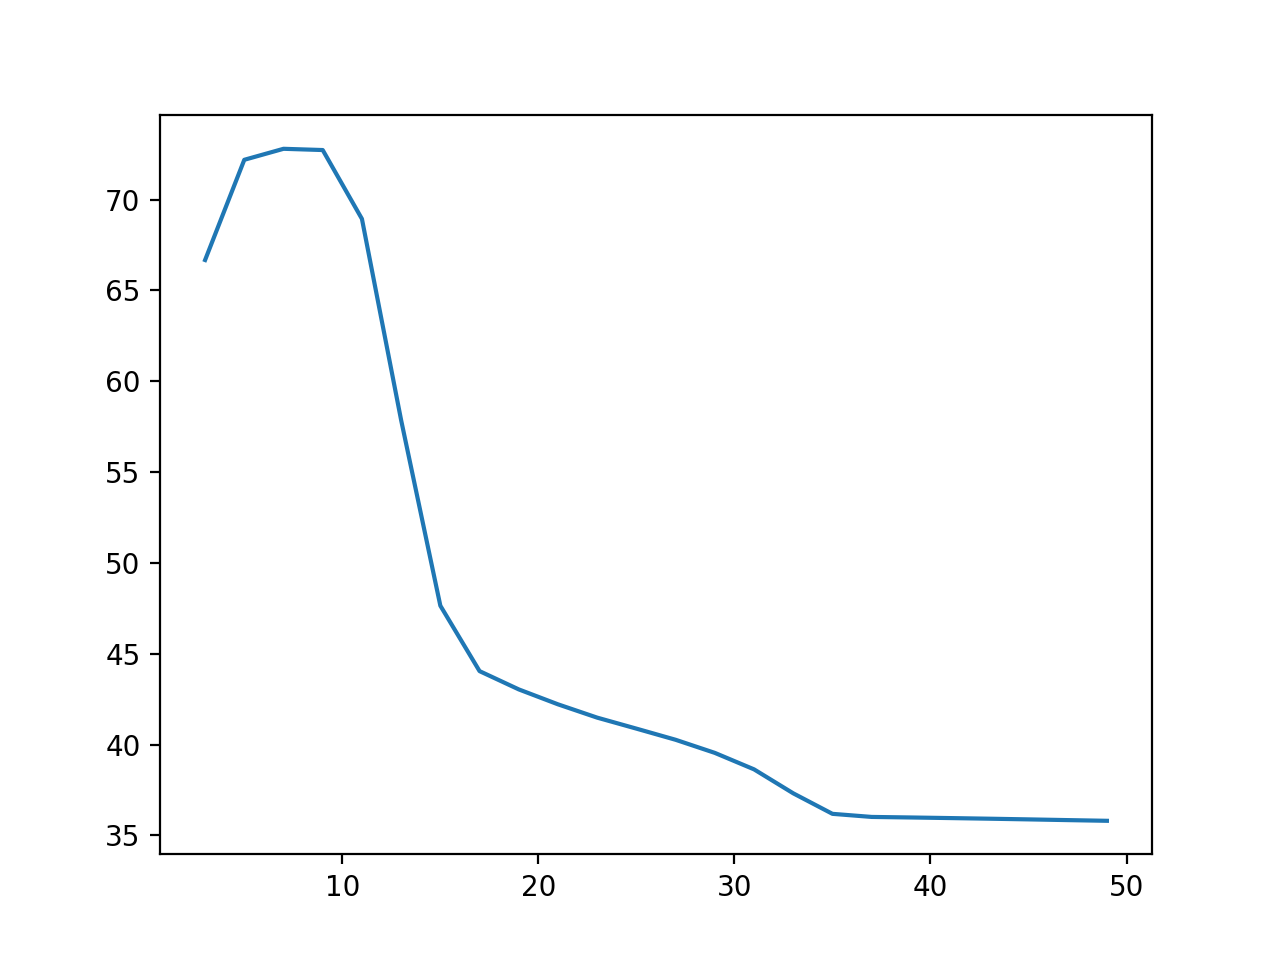
\includegraphics[scale=.45]{./basic_denoising/shepplogan/median_psnr_sp.png}
      \caption{PSNR vs filter size (Median)}
    \endminipage
    \end{figure}
    \pagebreak
% -------------------------------------------------------
% Complete

    
% -------------------------------------------------------
% -------------------------------------------------------
% Topic II
    \pagebreak
    \subsection*{Edge-Perserving Smoothing}
    I implemented the \textit{total variation denoising} and used it on the images from previous discussion. Also, followed are results from an example implementation of total variation.
    
    % Noisy Image
    \begin{figure}[!htb]
    \begin{center}
     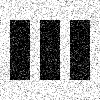
\includegraphics[scale=2.4]{./edge_preserving_smoothing/example/tv_noisy.png}
     \caption{Noisy Image}
    \end{center}
    \end{figure}
    
    % Recovered Image
    \begin{figure}[!htb]
    \begin{center}
     
\includegraphics[scale=2.4]{./edge_preserving_smoothing/example/tv_recovered.png}
     \caption{Recovered Image}
    \end{center}
    \end{figure}
    
    \pagebreak
% -------------------------------------------------------
% Complete
    \subsubsection*{Gaussian Noise Images}
    Here are the results of application of \textit{total variation filtering} on \textit{gaussian noise images} from before.
    
    \begin{figure}[!htb]
    \minipage{0.45\textwidth}
      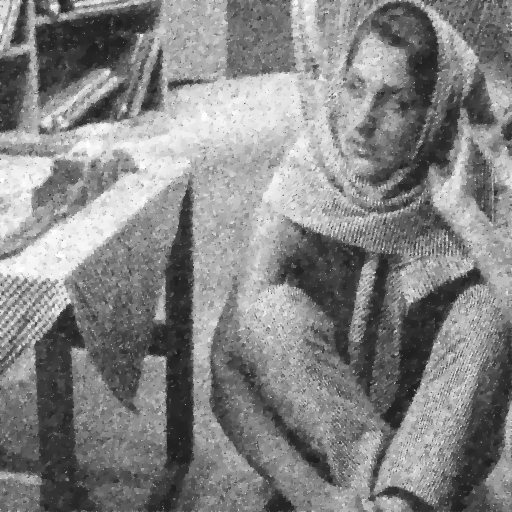
\includegraphics[scale=.45]{./edge_preserving_smoothing/barbara/gaussian.png}
      \caption{Barbara}
    \endminipage \hfill
    \minipage{0.45\textwidth}
      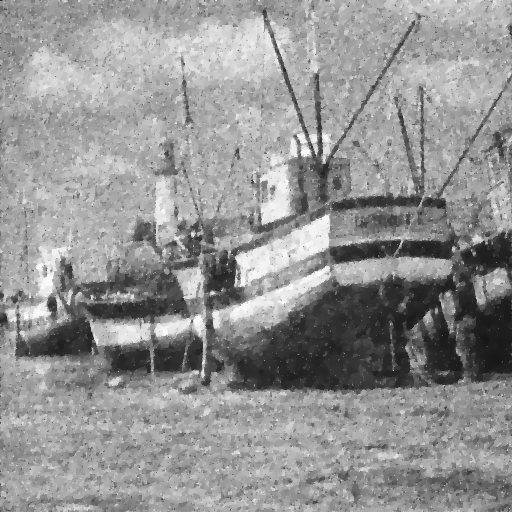
\includegraphics[scale=.45]{./edge_preserving_smoothing/boat/gaussian.png}
      \caption{Boat}
    \endminipage
    \end{figure}
    
    \phantom{}
    
    \begin{figure}[!htb]
    \minipage{0.45\textwidth}
      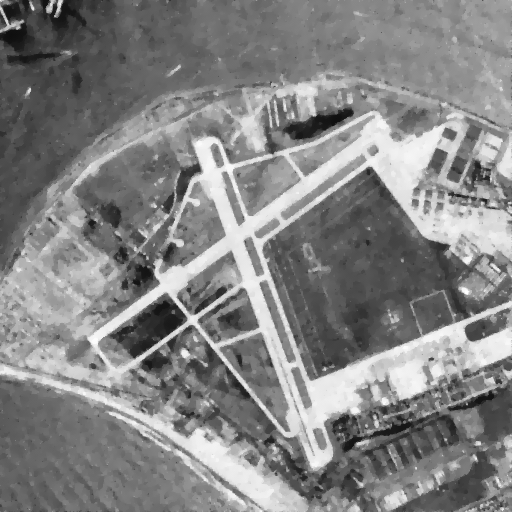
\includegraphics[scale=.45]{./edge_preserving_smoothing/sandiego/gaussian.png}
      \caption{Sandiego}
    \endminipage \hfill
    \minipage{0.45\textwidth}
      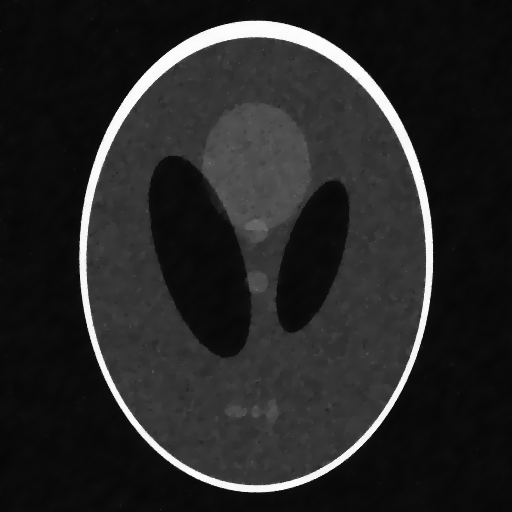
\includegraphics[scale=.45]{./edge_preserving_smoothing/shepplogan/gaussian.png}
      \caption{Shepplogan}
    \endminipage
    \end{figure}
    
    \pagebreak
% -------------------------------------------------------
% Complete
    \subsubsection*{Salt/Pepper Noise Images}
    Here are the results of application of \textit{total variation filtering} on \textit{salt/pepper noise images} from before.
    
    \begin{figure}[!htb]
    \minipage{0.45\textwidth}
      \includegraphics[scale=.45]{./edge_preserving_smoothing/barbara/sp.png}
      \caption{Barbara}
    \endminipage \hfill
    \minipage{0.45\textwidth}
      \includegraphics[scale=.45]{./edge_preserving_smoothing/boat/sp.png}
      \caption{Boat}
    \endminipage
    \end{figure}
    
    \phantom{}
    
    \begin{figure}[!htb]
    \minipage{0.45\textwidth}
      \includegraphics[scale=.45]{./edge_preserving_smoothing/sandiego/sp.png}
      \caption{Sandiego}
    \endminipage \hfill
    \minipage{0.45\textwidth}
      \includegraphics[scale=.45]{./edge_preserving_smoothing/shepplogan/sp.png}
      \caption{Shepplogan}
    \endminipage
    \end{figure}
    
    \pagebreak
% -------------------------------------------------------
% Complete

    
% -------------------------------------------------------
% -------------------------------------------------------
% Topic IIIA
    \subsection*{Deblurring}
    \subsubsection*{Variation in Noise}
    In this section, I focused on implementing the \textbf{Wiener Filtering Procedure} and applied on a set of \textit{blurred images}, with \textit{different noise variations}. The results are presented below. \\[10pt]
    % Noise 0
    \begin{figure}[!htb]
    \minipage{0.32\textwidth}
      \includegraphics[scale=.28]{./deblurring/0/final.png}
      \caption{\(\sigma\) = 0.0}
    \endminipage\hfill
    \minipage{0.32\textwidth}
      \includegraphics[scale=.28]{./deblurring/0/recover.png}
      \caption{Weiner Filtering}
    \endminipage\hfill
    \minipage{0.32\textwidth}%
      \includegraphics[scale=.28]{./deblurring/0/inverse.png}
      \caption{Inverse Filtering}
    \endminipage
    \end{figure}
    \\[5pt]
    % Noise 0.001
    \begin{figure}[!htb]
    \minipage{0.32\textwidth}
      \includegraphics[scale=.28]{./deblurring/0_001/final.png}
      \caption{\(\sigma\) = 0.001}
    \endminipage\hfill
    \minipage{0.32\textwidth}
      \includegraphics[scale=.28]{./deblurring/0_001/recover.png}
      \caption{Weiner Filtering}
    \endminipage\hfill
    \minipage{0.32\textwidth}%
      \includegraphics[scale=.28]{./deblurring/0_001/inverse.png}
      \caption{Inverse Filtering}
    \endminipage
    \end{figure}
    % Break
    \pagebreak
    \subsubsection*{Variation in Noise}
    With increase in noise, some more observations were made (listed below).\\[10pt]
    % Noise 0.01
    \begin{figure}[!htb]
    \minipage{0.32\textwidth}
      \includegraphics[scale=.28]{./deblurring/0_01/final.png}
      \caption{\(\sigma\) = 0.01}
    \endminipage\hfill
    \minipage{0.32\textwidth}
      \includegraphics[scale=.28]{./deblurring/0_01/recover.png}
      \caption{Weiner Filtering}
    \endminipage\hfill
    \minipage{0.32\textwidth}%
      \includegraphics[scale=.28]{./deblurring/0_01/inverse.png}
      \caption{Inverse Filtering}
    \endminipage
    \end{figure}
    \bigbreak
    \\[5pt]
    % Noise 0.1
    \begin{figure}[!htb]
    \minipage{0.32\textwidth}
      \includegraphics[scale=.28]{./deblurring/0_1/final.png}
      \caption{\(\sigma\) = 0.1}
    \endminipage\hfill
    \minipage{0.32\textwidth}
      \includegraphics[scale=.28]{./deblurring/0_1/recover.png}
      \caption{Weiner Filtering}
    \endminipage\hfill
    \minipage{0.32\textwidth}%
      \includegraphics[scale=.28]{./deblurring/0_1/inverse.png}
      \caption{Inverse Filtering}
    \endminipage
    \end{figure}\\[5pt]
    \begin{itemize}
        \item Inverse Filtering gives invalid results in case there's noise.
        \item The results obtained from Weiner Filtering get coarser as the noise increases.
    \end{itemize}
    \pagebreak

% -------------------------------------------------------
% Complete

    
% -------------------------------------------------------
% -------------------------------------------------------
% Topic IIIB
    \subsubsection*{Variation in Estimate}
    In the previous sections we used the original image spectrum \(F(u,v)\) as the \textit{estimate parameter} in \textit{weiner filtering.} Now in this section I tried some generic estimates for the image. The following results were observed.
    
    \begin{figure}[!htb]
    \minipage{0.45\textwidth}
      \includegraphics[scale=.45]{./deblurring/estimate/noisy.png}
      \caption{Noisy Image}
    \endminipage \hfill
    \minipage{0.45\textwidth}
      \includegraphics[scale=.45]{./deblurring/estimate/real.png}
      \caption{Real Image Estimate}
    \endminipage
    \end{figure}
    
    \phantom{}
    
    \begin{figure}[!htb]
    \minipage{0.45\textwidth}
      \includegraphics[scale=.45]{./deblurring/estimate/constant.png}
      \caption{Constant Image Estimate}
    \endminipage \hfill
    \minipage{0.45\textwidth}
      \includegraphics[scale=.45]{./deblurring/estimate/power.png}
      \caption{Power Estimate \(\alpha = 0.53\)}
    \endminipage
    \end{figure}

    \pagebreak
% -------------------------------------------------------
% Complete


    
% -------------------------------------------------------
% -------------------------------------------------------
% Topic IVB
    \subsection*{Real World Images}
    In this section we were supposed to use whatever we have learned so far, in trying to recover images from real world scenarios of blurring/noising.\\[1pt]
    
    % SHAN
    \textbf{Motion Blur I}\\
    The image provided was motion-blurred.\\[3pt]
    % Features
    \begin{figure}[!htb]
    \minipage{0.52\textwidth}
     \centering
      \includegraphics[scale=2.2]{./real_world/shan/uniform.png}
      \caption{Uniform Patch \((\sigma = 0)\)}
    \endminipage\hfill
    \minipage{0.52\textwidth}
    \centering
      \includegraphics[scale=3.5]{./real_world/shan/psf.png}
      \caption{PSF Estimate}
    \endminipage\hfill
    \end{figure}
    % Images
    \begin{figure}[!htb]
    \minipage{0.45\textwidth}
      \includegraphics[scale=1.25]{./real_world/shan/shan.png}
      \caption{Blurred Image}
    \endminipage\hfill
    \minipage{0.45\textwidth}
      \includegraphics[scale=0.3]{./real_world/shan/final.png}
      \caption{Recovered Image}
    \endminipage\hfill
    \end{figure}
    \pagebreak
    
    %Bharti
    \textbf{Defocus Blur I}\\
    The image provided was focus-blurred. The image was analysed in various ways to get the idea of \(H\) Spectrum and \(N\) Spectrum.\\[1pt]
    For getting the idea of noise, a uniform patch in the image (sky) was clipped and then analysed, which indicated the noise was as good as void.\\
    Then a (partial) edge in the image was analysed, where the gradient of values gave the idea of spread of blurring. A good approximate was a disc shaped spatial filter\\
    % Features
    \begin{figure}[!htb]
    \minipage{0.45\textwidth}
     \centering
      \fbox{\includegraphics[scale=3.3]{./real_world/bharti/uniform.png}}
      \caption{Uniform Patch \((\sigma = 0)\)}
    \endminipage\hfill
    \minipage{0.45\textwidth}
    \centering
      \includegraphics[scale=0.45]{./real_world/bharti/gradient.png}
      \caption{Gradient}
    \endminipage\hfill
    \end{figure}
    \bigbreak
    % Images
    \begin{figure}[!htb]
    \minipage{0.45\textwidth}
      \includegraphics[scale=0.35]{./real_world/bharti/bharti.png}
      \caption{Blurred Image}
    \endminipage\hfill
    \minipage{0.45\textwidth}
      \includegraphics[scale=0.35]{./real_world/bharti/final.png}
      \caption{Recovered Image}
    \endminipage\hfill
    \end{figure}
    \pagebreak
    
    % Yuzhikov
    \textbf{Defocus Blur II}\\
    Working out this image involved the same steps as above, except for that the best approximation for the filter was a disc based function with radius 8.
    \begin{figure}[!htb]
    \minipage{0.45\textwidth}
      \includegraphics[scale=0.33]{./real_world/yuzhikov/yuzhikov.png}
      \caption{Blurred Image}
    \endminipage\hfill
    \minipage{0.45\textwidth}
      \includegraphics[scale=0.3]{./real_world/yuzhikov/final.png}
      \caption{Recovered Image}
    \endminipage\hfill
    \end{figure}
    
    \subsubsection*{Note}
    In the case of defocus blur, we observe that ringing is prominent. This may arise from the fact that since the disc function have abrupt cuts, which leads to ringing in the fourier domain, and thus edges resonates rings.\\
    Also to eliminate unnecessary ringing from considering the periodic image (i.e. totally different pixel values once the image is repeated), I blurred the image borders with the wrapped around images. This caused significant decrease in ringing in recovered images.
    \pagebreak
% -------------------------------------------------------
% Complete

% -------------------------------------------------------
% -------------------------------------------------------
    % Noise Analysis
    \subsection*{Noise Analysis}
    Starting with \textit{gaussian noise} with std. dev. \(\sigma\) (assuming mean \(\mu = 0\)) and shape \((M,N)\). \\
    Now, \(\sum n(x, y)^2 = \sum |n(x, y) - \mu|^2 = \sigma^2 * M * N\) \\
    And, thus our noise spectrum magnitude becomes (in spatial domain) \(\sigma^2 * M * N\).\\
    Also, from the property of fourier transform, \(\sum |n(x, y)|^2 = \frac{1}{MN}*\sum |N(u,v)|^2\), \\
    we get that, \(\sum |N(u, v)|^2 = \sigma^2 * M^2 * N^2\). \\
    
    \begin{table}[]
    \centering
    \begin{tabular}{c|c|c}
    \(\sigma\) & \(\sum |N(u, v)|^2\) & {\(\frac{\sum |N(u, v)|^2}{\sigma^2 * M^2 * N^2}\)} \\
        0.1 & 688280680.32 &{1.0015} \\
        0.01 & 6905896.64 &{1.0049} \\
        0.001 & 68811.47 &{1.0013}
    \end{tabular}
    \end{table}

% -------------------------------------------------------
% Complete


% -------------------------------------------------------
% -------------------------------------------------------
    % Conclusion
    \subsection*{Observations}
    Following were the major observations for sub-parts.
    \begin{itemize}[topsep=0cm]
        \item \textbf{Mean filter} works better on \textit{gaussian noise} and \textbf{Median filter} works best on \textit{S/P} noise.
        \item \textbf{Total Variation} works amazingly well on \textit{gaussian noise}, but fails to give promising results in \textit{S/P} noise. This is perhaps due to consideration of \(Laplacian\) operator which in case of S/P isn't of much use.
        \item \textbf{Weiner filtering} works best with \textit{original image} as the estimate. Also, restoration is much better when the noise is low.
    \end{itemize}

    \subsection*{Summary}
    All required by the assignment was implemented and a lot of new things were learned/understood. The codes are written in Python. All the functions were implemented on own (except for the FFT, which was allowed to be used). \\
    The code was patterned as a library of functions, which can be used on any Python interpreter in a series of steps to give the desired solution. (for assignment)\\
    The assignment was intriguing and I learnt a lot of new ideas. Thanks and Regards.
    
\end{document}